%------------------------------------------------------------------------------
% Template file for the submission of papers to IUCr journals in LaTeX2e
% using the iucr document class
% Copyright 1999-2013 International Union of Crystallography
% Version 1.6 (28 March 2013)
%------------------------------------------------------------------------------

\documentclass{iucr}              % DO NOT DELETE THIS LINE
% \documentclass[preprint]{iucr}              % DO NOT DELETE THIS LINE

\usepackage{epsfig,color}
\usepackage{graphicx}
\usepackage{amsmath,amssymb}


% \documentclass[a4paper,10pt]{article}
% \usepackage[utf8]{inputenc}
% \usepackage[]{graphicx}
% \usepackage{rotating}
% \usepackage{hyperref}
% \usepackage{amsmath} 
% \usepackage{color}
% \usepackage{listings}
% \usepackage{lscape}
% \usepackage{float}
% \usepackage{verbatim}

% \usepackage{subcaption}
% \usepackage{multirow}


\def\ave#1{{\langle #1\rangle}}
\def\half{{1\over 2}}

\newcommand{\refeq}[1]{Eq.~\ref{#1}}
\newcommand{\refpic}[1]{Fig.~\ref{#1}}
\newcommand{\todo}[1]{{\color{red}[TODO: "#1'']}}
\newcommand{\reftable}[1]{Table.~\ref{#1}}
\newcommand{\inblue}[1]{{\color{blue}#1}}
\newcommand{\inred}[1]{{\color{red}#1}}
\newcommand{\ingreen}[1]{{\color{green}#1}}

\DeclareMathOperator{\sinc}{sinc}
% \lstset{language=Python,
%         keywordstyle=\color{blue}\textbf,
% 	commentstyle=\color[rgb]{0.133,0.545,0.133},
% 	stringstyle=\color[rgb]{0.627,0.126,0.941},
% 	breaklines=true,
% 	showstringspaces=false,
% 	frame=trBL, basicstyle=\scriptsize %\small %\tiny %\footnotesize
%        }




     %-------------------------------------------------------------------------
     % Information about journal to which submitted
     %-------------------------------------------------------------------------
     \journalcode{S}              % Indicate the journal to which submitted
                                  %   A - Acta Crystallographica Section A
                                  %   B - Acta Crystallographica Section B
                                  %   C - Acta Crystallographica Section C
                                  %   D - Acta Crystallographica Section D
                                  %   E - Acta Crystallographica Section E
                                  %   F - Acta Crystallographica Section F
                                  %   J - Journal of Applied Crystallography
                                  %   M - IUCrJ
                                  %   S - Journal of Synchrotron Radiation

\begin{document}                  % DO NOT DELETE THIS LINE

     %-------------------------------------------------------------------------
     % The introductory (header) part of the paper
     %-------------------------------------------------------------------------

     % The title of the paper. Use \shorttitle to indicate an abbreviated title
     % for use in running heads (you will need to uncomment it).

\title{A hierarchical approach for modelling X-ray beamlines. Application to a coherent beamline.}

     % Authors' names and addresses. Use \cauthor for the main (contact) author.
     % Use \author for all other authors. Use \aff for authors' affiliations.
     % Use lower-case letters in square brackets to link authors to their
     % affiliations; if there is only one affiliation address, remove the [a].

\cauthor[a]{Manuel}{Sanchez del Rio}{srio@esrf.eu}{}
\author[a]{Rafael}{Celestre} %{address if different from \aff}
\author[a]{Mark}{Glass} %{address if different from \aff}
\author[a]{Giovanni}{Pirro} %{address if different from \aff}
\author[a]{Juan}{Reyes Herrera} %{address if different from \aff}
\author[a]{Ray}{Barrett} %{address if different from \aff}
\author[a]{Julio Cesar}{da Silva} %{address if different from \aff}
\author[a]{Peter}{Cloetens} %{address if different from \aff}
\author[b]{Xianbo}{Shi}
\author[b]{Luca}{Rebuffi}


\aff[a]{ESRF, 71 Avenue des Martyrs, 38043 Grenoble \country{France}}
\aff[b]{Argonne National Laboratory, 9700 South Cass Avenue, Lemont, Illinois 60439, \country{USA}}


     % Use \shortauthor to indicate an abbreviated author list for use in
     % running heads (you will need to uncomment it).

%\shortauthor{Soape, Author and Doe}

     % Use \vita if required to give biographical details (for authors of
     % invited review papers only). Uncomment it.

%\vita{Author's biography}

     % Keywords (required for Journal of Synchrotron Radiation only)
     % Use the \keyword macro for each word or phrase, e.g. 
     \keyword{Beamline}\keyword{simulations}

%\keyword{keyword}

     % PDB and NDB reference codes for structures referenced in the article and
     % deposited with the Protein Data Bank and Nucleic Acids Database (Acta
     % Crystallographica Section D). Repeat for each separate structure e.g
     % \PDBref[dethiobiotin synthetase]{1byi} \NDBref[d(G$_4$CGC$_4$)]{ad0002}

%\PDBref[optional name]{refcode}
%\NDBref[optional name]{refcode}


\maketitle                        % DO NOT DELETE THIS LINE

\begin{synopsis}
A hierarchical scheme of the calculations of an X-ray beamline for coherent applications is presented. Starting from simple calculations to partial coherence calculations, we show how ray tracing and wave optics software are applied simulating the beamline performances.   
\end{synopsis}

\begin{abstract}
We consider different approaches to simulate a modern X-ray beamline. Several methodologies with increasing complexity are applied to discuss the relevant parameters that quantify the beamline performances. Parameters such as flux, beam size at the image and coherence properties are obtained from simple analytical calculations to sophisticated computer simulations using ray tracing and waveoptics techniques. A last generation x-ray nanofocusing beamline for coherent  applications (ID16A at the ESRF) has been chosen  to study in detail the issues 
related to highly demagnifying sychrotron sources and exploiting the beam coherence. The performance of the beamline is studied for two storages rings: the old ESRF (emittance 4000 pm) and the new ESRF-EBS (emittance 150 pm). In addition to traditional results in term of flux, intensity distribution and focal size, an innovative study on the partial coherence properties based on propagation of coherent modes is presented. The different algorithms and methodologies are implemented in the software suite OASYS \cite{codeOASYS}. They are discussed with emphasis in benefits and limitations of each one. 
\end{abstract}


     
\section{Introduction}


Many storage ring based x-ray synchrotron facilities are building or planning upgrades to increase brilliance and coherent flux by one to three orders of magnitude.  The first upgrade of a large facility will be the EBS (Extremely Brilliant Source) \cite{orangebook} at the European Synchrotron Radiation Facility (ESRF), aiming to build a storage ring of 150 pm emittance to significantly boost the associated x-ray coherence. Applications exploiting beam coherence such as such as x-ray photon correlation spectroscopy, coherent diffraction imaging, propagation-based phase contrast imaging and ptychography will strongly benefit from this update.  

Accurate calculation and quantitative evaluation of the parameters related to x-ray optics is of paramount importance for designing, building and exploiting the new beamlines. Every modern beamline follows a procedure of conceptual design and then technical design where detailed simulations are essential. The calculations allow the designer to test the design parameters in a virtual computer environment where pros and cons can be studied quantitatively. The selection to the best performant optics configuration requires the detailed simulation of the optics imperfections, that in many cases are the limiting factor of the beamline optical configuration. Deformation in the optical elements due to heat load need to be controlled, therefore optics simulations have to include results from engineering modeling of the thermal deformation associated to mechanical issues usually dome using finite eelement analysis. Traditionally the optics calculations for synchrotron beamlines are done using ray tracing techniques. They model the x-ray beam as a collection of different rays that are incoherent one to another. This technique is still essential for obtaining information on aberrations, flux propagation, monochromator bandwidth, etc. However, the high coherence of the new sources make necessary to complement the ray tracing methods with models including effects of diffraction and scattering from a coherent beam. A fully coherent beam is still a dream for the new generation storage rings. In spite of a high increate of the coherent fraction of the new beams, the coherent fraction at tipically hard x-ray photon energies is still at few percent for the new sources. This makes still important a ray tracing analysis that does not become obsolete, but has to be complemented with an analysis based on wave optics. Because of the non perfect coherence the wave optics analysis becomes non trivial and can be done with different levels of approximation, as discussed in this work. In addition, wave optics simulations are usually expensive from the computer point of view.

For illustrating the applicability of a battery of methods and solutions for beamline optics simulations we have chosen the ESRF beamline ID16A. This beamline provides a high-brilliance beam focused to a few nanometer. It shows characteristics increasingly searched in modern beamlines: extremely high demagnification (sub-micrometer beam) and high coherence. It combines coherent imaging techniques and X-ray fluorescence microscopy to perform quantitative 3D characterization of the morphology and the elemental composition of specimens in their native state \todo{complete ID16A description}. 

X-ray beamlines are very particular optical systems. Some implications of exploiting low wavelengths such as the necessity of using grazing incidence reflectors and the use of perfect crystals as typical hard x-ray monochromators make useless, or at least incomplete, the application of common commercial software packages for the study of synchrotron beamlines. For this reason many optics tools have been developed by the synchrotron community. Some of them have a long history like SHADOW (more than 40 years old) or SRW (almost 30), for mentioning only codes used in this work. These historical tools together with new tools designed ad-hoc packages have been agglutinated in a user friendly software OASYS. Many of the calculations presented here have been performed directly in OASYS or with script created with the help of OASYS. 


The paper is structures as follows: we first introduce in Section~\ref{Beamline description} the main parameters of the beamline and make the selection of the particular choice of the parameters used in the calculations. Section~\label{Simulations} is the central part of the paper, and describe the different methods used to analyse the beamline with increasing complexity, setting a hierarchy of methodologies that can be exported to the simulations of any beamline. In Section \ref{level0} we calculate with simple methods approximated values of focal size, flux and coherent fraction. Then accuracy is improved using geometrical methods in Section \ref{level1} that give reasonable results as far as some corrections are considered because of the  mentioned characteristics of high demagnification and high coherence of the studied beamline. The wave optics section~]ref{level2} also include different models whose complexity increases when the results expected are more and mode demanding. The simulations methods are presented in a hierarchical approach:  they provide more and better results but the price to pay is to deal with more complex and computationally expensive tools. 

 %-------------------------------------------------------------------------
 % Manuel & Rafael
 %-------------------------------------------------------------------------

\section{Beamline description}
\label{Beamline description}

This section presents the reader with the main operational parameters for the ID16A beamline at ESRF in two scenarios. This beamline was built during the Upgrade Phase I at ESRF in \inred{2011??}. It uses one or several undulators as source. During the period 2011-2018 it worked exploiting the ESRF storage ring’s double-bend achromat (DBA) lattice with horizontal emittance about 4000 pm. The replacement of this lattice by a new hybrid multi-bend achromat (HMBA) lattice is being achieved in the ESRF Upgrade Phase II. This new lattice will drastically improve the performances of the ESRF source. The result, the Extreme Brilliant Source (EBS) \cite{orangebook} will increase the brightness and coherent fraction by a factor of more than 100, by strongly reducing the horizontal emittance. This is possible using almost the same ring circunference and electron energy $E_e$. As as result, the x-ray sources will be much coherent, specially in the horizontal direction. This work shows some quantitative results on how the storage ring upgrade will affect a particular beamline is analyzed in this paper. 

ID16A \cite{ID16A} is a bemline that provides a nanometric, highly coherent, pink beam. It is dedicated to nanofocusing applications. \todo{please summarize some use and application}. The beamline usually operates at three fixed photon energies: 11200 eV, 17225 eV and 33600 eV. The straight section in the magnet lattice holds three undulators: an in-vacuum undulator of $\lambda_u=26$~mm period, and two other conventional undulators of 18 and 22.4 mm period. The undulator parameters and $K$-values at the resonances for the energies in use are shown in Table \ref{tab:Undulators}. 

\begin{table}\label{tab:Undulators}
\centering
\caption{Parameters of the undulators available at the ID16A beamline: period ($\lambda_u$), length ($L$), number of identical undulators ($N$) and deflection parameter ($K$) values for the three main photon energies in use. The valuse are shown for the two ESRF magnetic lattices: the old one (labelled ESRF, with $E_e = 6.04$ GeV) and the new one (EBS, with $E_e = 6.00$ GeV). $n$ is the emission harmonic in use for each particular photon energy.}

\resizebox{\textwidth}{!}{%
\begin{tabular}{lcccccc}
name  & $\lambda_u$ [mm] & $L$ [m] & N & $K$ (11200 eV) & $K$ (17225 eV) & $K$ (33600 eV) \\ 
\input{tableUndulator.txt}
%      & IVU26 & 26.00           & 2.50    & 1      & 0.616 (n=1)    & 1.625 (n=3)    & 0.616 (n=3)    \\
% ESRF & U18.3 & 18.30           & 1.40    & 2      & 1.715 (n=1)    & 0.445 (n=1)    & 1.715 (n=3)    \\
%      & U22.4 & 22.40           & 1.40    & 1      & 0.873 (n=1)    & 1.840 (n=1)    & 0.873 (n=1)    \\ \hline
%      & IVU26 & 26.00           & 2.50    & 1      & 0.590 (n=1)    & 1.606 (n=1)    & 0.590 (n=3)    \\
% EBS  & U18.3 & 18.30           & 1.40    & 2      & 1.156 (n=1)    & 0.411 (n=1)    & 1.156 (n=1)    \\
%      & U22.4 & 22.40           & 1.40    & 1      & 0.852 (n=1)    & 1.821 (n=3)    & 0.852 (n=1)    \\ \hline
\end{tabular}%
}
\end{table}

ID16A is a long beamline (the distance from the center of the straight section to the sample position is 185 m). A strong focusing is performed with a Kirkpatrick-Baez (KB) set of mirrors placed very close (a few cm) upstream the sample position (focal plane), which ensures a high demagnification. In order to match the acceptance of the KB in the vertical and horizontal planes a focusing multilayer monochromator (ML) has
been chosen. It i) monochromatises the beam with a large energy bandwidth (typically $\Delta E/E \approx 10^{-2}$) to allow high (pink) flux, 
and ii) creates a secondary secondary source in horizontal plane 40 m downstream from the undulator, where a horizontal slit (VSS, virtual source slit) is placed. A beamline schematic is shown in Figure~\ref{fig:ID16A}. The positions of the different elements are shown in Table \ref{tab:Positions}. This table also shows the extremely high geometrical demagnification ($\sim 10^3$) needed for focusing the beam to the nanometric range.  

\begin{figure}\label{fig:ID16A}
    \centering
    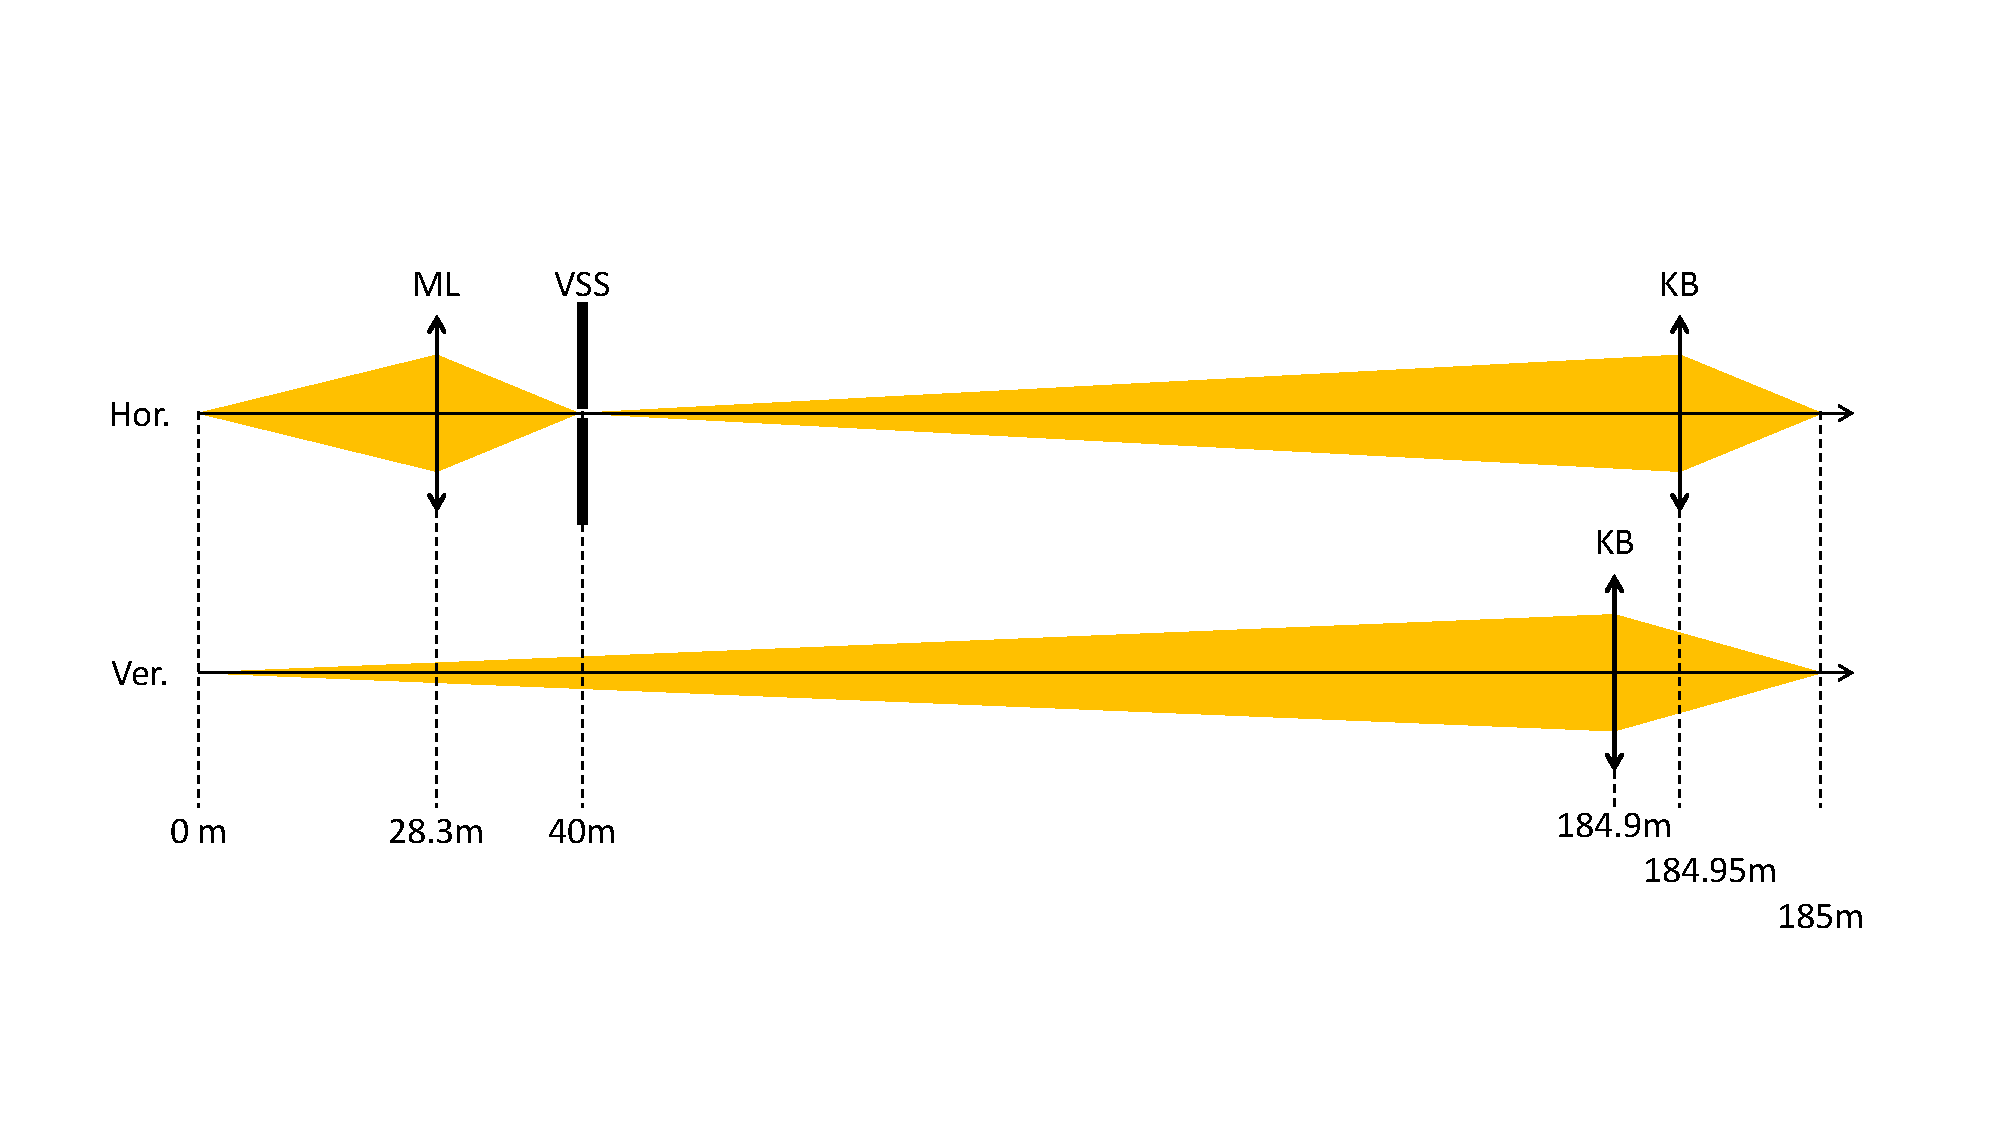
\includegraphics[width=0.9\textwidth,clip=true,trim=50 85 50 85]{GRAPHICS/ID16A.pdf}
    \caption{Schematic of the ID16A beamline showing the horizontal (top) and vertical (bottom) planes and the position of the main optical elements. In the sketch ML stands for the focusing multilayer monochromator; VSS for virtual source slit; and KB for the Kirkpatrick-Baez set of mirrors. The sketch is drawn out of scale.}
\end{figure}


\begin{table}\label{tab:Positions}
    \caption{Position of the main ID16A optical elements with respect to the source (undulator centre). It also shows the values for horizontal and vertical demagnification $M^{-1}=p/q$, where $p$ and $q$ are the the distances object-optics and optics-image, respectively.}
    \resizebox{\textwidth}{!}{%
    \begin{tabular}{rcccccc}
    -                      & Source & Multilayer & Slit  & KB (v) & KB (h) & Focal plane \\ 
    Position {[}m{]}:      & 0.00   & 28.30      & 40.00 & 184.90 & 184.95 & 185.00      \\
    Horizontal $M^{-1}$:   & -      & 2.42       & -     & -      & 2899   & -           \\
    Vertical $M^{-1}$:     & -      & -          & -     & \inblue{1849}   & -      & -           \\ 
    \end{tabular}%
    }%
\end{table}


Simulations were done using the two different storage ring lattices mentioned before: the (present) ESRF DBA where the undulators are in a high-$\beta$ straight section (larger horizontal emittance) and the new EBS (lower horizontal emittance) straight sections. The parameters for the current and the new lattice are shown in Tables \ref{tab:TableSources} and \ref{tab:eBeam}.

\begin{table}\label{tab:TableSources}
    \caption{ESRF and ESRF-EBS main storage ring parameters. Main parameters of the present DBA lattice (ESRF) and future HMBA lattice (EBS) storage rings \cite{orangebook}.}
        \begin{tabular}{rcc}
                                              & \textbf{ESRF} & \textbf{EBS}      \\ 
        Lattice type:                         & DBA           & HMBA              \\
        Circunference {[}m{]}:                & 844.930       & 843.979           \\
        Beam energy {[}GeV{]}:                & 6.04          & 6.00              \\
        Beam current {[}mA{]}:                & 200           & 200               \\
        Natural emittance {[}pm$\cdot$rad{]}: & 4000          & 147               \\
        Energy spread {[}$\%${]}:             & 0.0011        & 0.00093           \\       
    \end{tabular}
\end{table}

\begin{table}\label{tab:eBeam}
    \centering
    \caption{ESRF and EBS main electron beam parameters. Electron beam parameters for the high-$\beta$ (ESRF) and the EBS straight sections. Values taken at the symmetry point of the straight section, where the insertion devices are placed. Values fir ESRF are taken from \cite{ESRF2014}. For EBS, two (very close) design values are used, from Ref.~\cite{ESRF2014} labelled EBS-S28A, and those coming from further lattice refinement, labelled EBS-S28D. \todo{Remove ESRF-AT?? Check again} }
        \resizebox{\textwidth}{!}{%
        \begin{tabular}{ccccc}
         Lattice & $\sigma_e$ horizontal {[}$\mu$m{]} &  $\sigma_e'$ horizontal {[}$\mu$rad{]} & $\sigma_e$ vertical {[}$\mu$m{]} & $\sigma_e'$ vertical {[}$\mu$rad{]} \\
         \input{tableElectron.txt}

%    \begin{tabular}{rcc}
%                                                & \textbf{ESRF (high-$\beta$)} & \textbf{EBS}     \\ 
%         $\sigma_e$ horizontal {[}$\mu$m{]}:    & 415.00                      & 30.20             \\
%         $\sigma_e'$ horizontal {[}$\mu$rad{]}: & 10.30                       & 4.40              \\
%         $\sigma_e$ vertical {[}$\mu$m{]}:      & 3.40                        & 3.60              \\
%         $\sigma_e'$ vertical {[}$\mu$rad{]}:   & 1.20                        & 1.40              \\ 
    \end{tabular}
    }
\end{table}

\section{Simulations}

For all simulations presented hereafter, we selected the configuration using a single undulator U18.3 placed in the center of the straight section and tuned to its first harmonic at a photon energy of $E=17225$ eV (Table \ref{tab:Undulators}). This section is devided in three subsections, that present three main levels of simulations: simple calculations that can be made by hand (section \ref{level0}), ray-tracing simulations (section \ref{level1}) and wave optics simulations (section \ref{level2}).   

\subsection{Analytical calculations}
\label{level0}

We first estimate the beam size at different positions at the beamline, in particular at the source plane and at the image plane. A first na{\"{i}}ve estimation of the focal size can be done by considering the source size times the magnification factor $M$. In the paraxial approximation, the magnification factor can be expressed as $M=q/p$, where $p$ is the distance between object and imaging element and $q$ is the distance between imaging element and image. The demagnification is the inverse of the magnification ratio: $M^{-1}=p/q$. Systems where $M>1$ are said to be magnifying, whereas systems with $M<1$ (or $M^{-1}>1$) are said to be demagnifying. The latter will be our case, thus is more convenient to work with demagnification ($M^{-1}>1$) rather than with magnification. 

The source size is usually approximated supposing a Gaussian distribution of the electron sizes (or divergence) (Table \ref{tab:eBeam}) and undulator natural source size or divergence. Although the former is true, the latter is not. Let $\sigma_{e(h,v)}$ and $\sigma_{e(h,v)}'$ be the electron beam size and divergence at a centre of the symmetry of the straight section. The subscripts $h$ and $v$ stand for horizontal and vertical, respectively. The undulator natural source size and divergence are given by \cite{elleaume}:
\begin{align}
    \label{eq:photon small sigmas}
    \sigma_u=\frac{2.74}{4\pi}\sqrt{\lambda L}\approx \sqrt{\frac{\lambda L}{2 \pi^2}}  && \sigma_u' = 0.69\sqrt{\frac{\lambda}{L}}\approx \sqrt{\frac{\lambda}{2 L}},
\end{align}
where $\lambda$ is the emitted wavelength and $L=N\lambda_u$ is the undulator length, with $\lambda_u$ as the magnetic period of the undulator and $N$, the number of magnetic periods. The electron beam usually presents different horizontal and vertical beam emittances, but the undulator natural source size or divergence presents radial symmetry at the central cone (excluding polarization). The photon source size and divergence are given by the convolution of the electron sizes and the undulator natural sizes. If we consider Gaussian distributions, the photon source is
\begin{align}
\label{eq:photon big sigmas}
\Sigma_{h,v}=\sqrt{\sigma_{e(h,v)}^2 + \sigma_u^2} && \Sigma_{h,v}'=\sqrt{\sigma_{e(h,v)}'^2 + \sigma_u'^2}.
\end{align}

% $\Sigma$ is given by the convolution of the electron beam size and the undulator natural source size or equivalently, single electron source size \cite{elleaume}: a storage ring with low emittance will produce small photon source size. It is also convenient to define two other relationships: the first one relates the magnetic field $B$ in an undulator to a dimensionless parameter $K$, the deflection parameter: $K = 93.4\lambda_u[\text{m}]\text{B}[\text{T}]$. The second relationship shows the wavelengths at which the emitted spectral intensity os peaked, or resonance. It is a function of $K$; the harmonic number n; the Lorentz factor $\gamma$ and the observation angle $\phi$:
% \begin{align}
%     \lambda=\frac{\lambda_u}{2\text{n}\gamma^2}\Big(1+\frac{K^2}{2}+\gamma^2\phi^2\Big).
% \end{align}
% The first term is the relativistic contracted wavelength, the second term is the magnetic tuning and the last term is the off-axis wavelength increase \cite{elleaume}.

The beam sizes at different positions at the beamline were estimated in a different way depending if the beam is focused or not. If the beam is focused, its dimensions in a first approximation are the photon source size multiplied by the corresponding magnification factor. For predicting the photon beam in a non-focal position the beam divergence is used. In an ideal {\'{e}}tendue preserving optical system, where the conservation of the Smith-Helmholz invariante applies, the resulting beam divergence transforms inversely as the beam size: it can be calculated as the product between the beam divergence at the source with the demagnification factor $M^{-1}$.

Using the values for U18.3, $n$=1, and  $E=17225$ eV (Table \ref{tab:Undulators}), one obtains a focal size 139$\times$5 nm$^2$ (H$\times$V) for ESRF and 10$\times$5 nm$^2$ for EBS (Table~\ref{tab:HandCalculations}). The focal spot for ESRF lattice is too large in horizontal for the beamline specification, therefore the VSS could be closed to 50$\mu$m thus reducing the beamsize at the VSS plane by a factor ca. 8 \inred{$\approx$ 403.8/50=8.076}. Therefore the horizontal size at the sample will be affected by the same factor obtaining roughly 17$\times$5 nm$^2$

In general, for grazing incident optics with large demagnifications ($M^{-1} \gg 100$) imaging extended sources, the effect of optical aberrations is very important even using a perfect optical surface that focus point-to-point. As a consequence, the results calculated using only the demagnification factor are usually too optimistic. Moreover imperfections in the optical surface (figure errors, slope errors and microroughness) are often the limiting factors of the real reflective optics. Their effect will studied in Sections~\ref{level1} and \ref{level2}. The smearing of the focal size because of diffractive effects by the mirror clipping will also be discussed. 

\begin{table}\label{tab:HandCalculations}
    \centering
    \caption{Photon beam size and divergence for selected ID16A beamline positions. Values below were obtained considering undulator U18.3 tuned to its first harmonic at the photon energy of $E=17225$ eV for both the high-$\beta$ (ESRF) and the EBS straight sections. Values are FWHM. Values in parentheses corresponds to closing the VSS slit to 50$\mu$m (21.3 if approximating by the Gaussian $\sigma$).}
    \resizebox{\textwidth}{!}{%
    \begin{tabular}{r|ccc|ccc}
                            &               & \textbf{ESRF (high-$\beta$)} &   &         & \textbf{EBS}  &    \\ 
    Element:                & Undulator     & VSS          & Sample            & Undulator & VVS   & Sample       \\
    Position [m]:           & 0.00          & 40.00        & 185.00            & 0.00    & 40.00   & 185.00       \\
    $FWHM_h$ [$\mu$m]:      & 977.19        & 404.00 (50.0)& 0.139 (0.017)     & 71.26   & 29.46   & 0.0102       \\
    $FWHM_v$ [$\mu$m]:      & 9.60          & 482          & 0.0052            & 10.02   & 486.5   & 0.0054       \\
    \newline
    $FWHM'_h$ [$\mu$rad]:   & 26.96         & \inred{65.22?}        & 189062   & 15.60   & 37.74   & 109404       \\
    $FWHM'_v$ [$\mu$rad]:   & 12.04         & 12.04                 & 22264    & 12.16   & 12.16   & 22489        \\                                                   
    \end{tabular}%
    }
\end{table}

The next step would be to estimate the number of photons at the sample. For that, we need the spectrum at the source. It is not straightforward to get this information analytically but one can calculate the flux and power using different codes. Perhaps the most performant and well maintained codes spread in the synchrotron community are SPECTRA \cite{codeSPECTRA} and SRW \cite{codeSRW}. The XOPPY package in the OASYS suite implements three codes: US\cite{codeUS}, URGENT: \cite{codeURGENT} and SRW \cite{codeSRW}. Figure~\ref{fig:FluxU18} shows the spectra calculated over an aperture if 1 $\times$ 1 mm$^2$ placed at $d$=27.1 m. This aperture opening is set to fully accept the central cone at the resonance peak of the harmonic in use ($\max(\Sigma') \times d = 0.73$ mm), with $\Sigma'$ values from in Table~\ref{tab:HandCalculations}. The peak intensity is about  $2.9\cdot10^{14}$ photons/s/0.1{\%}bw for EBS and 1.9 10$^{14}$ for ESRF (see \ref{fig:FluxU18}). One can appreciate how the emittance plays an important role in both peak width and specially in peak amplitude. The number of photons per second after the multilayer monochromator is 2.9 10$^{14}$ for EBS and 1.9 10$^{14}$ for ESRF, considering that the energy bandwidth transmitted by a multilater monochromator is $\Delta E/E \approx 10^{-2}$ and the bandwidth in \ref{fig:FluxU18} is 10$^{-3}$, and supposing at this point ideal reflectivity (100\%) for the multilayers. 

\begin{figure}\label{fig:FluxU18}
    \centering
    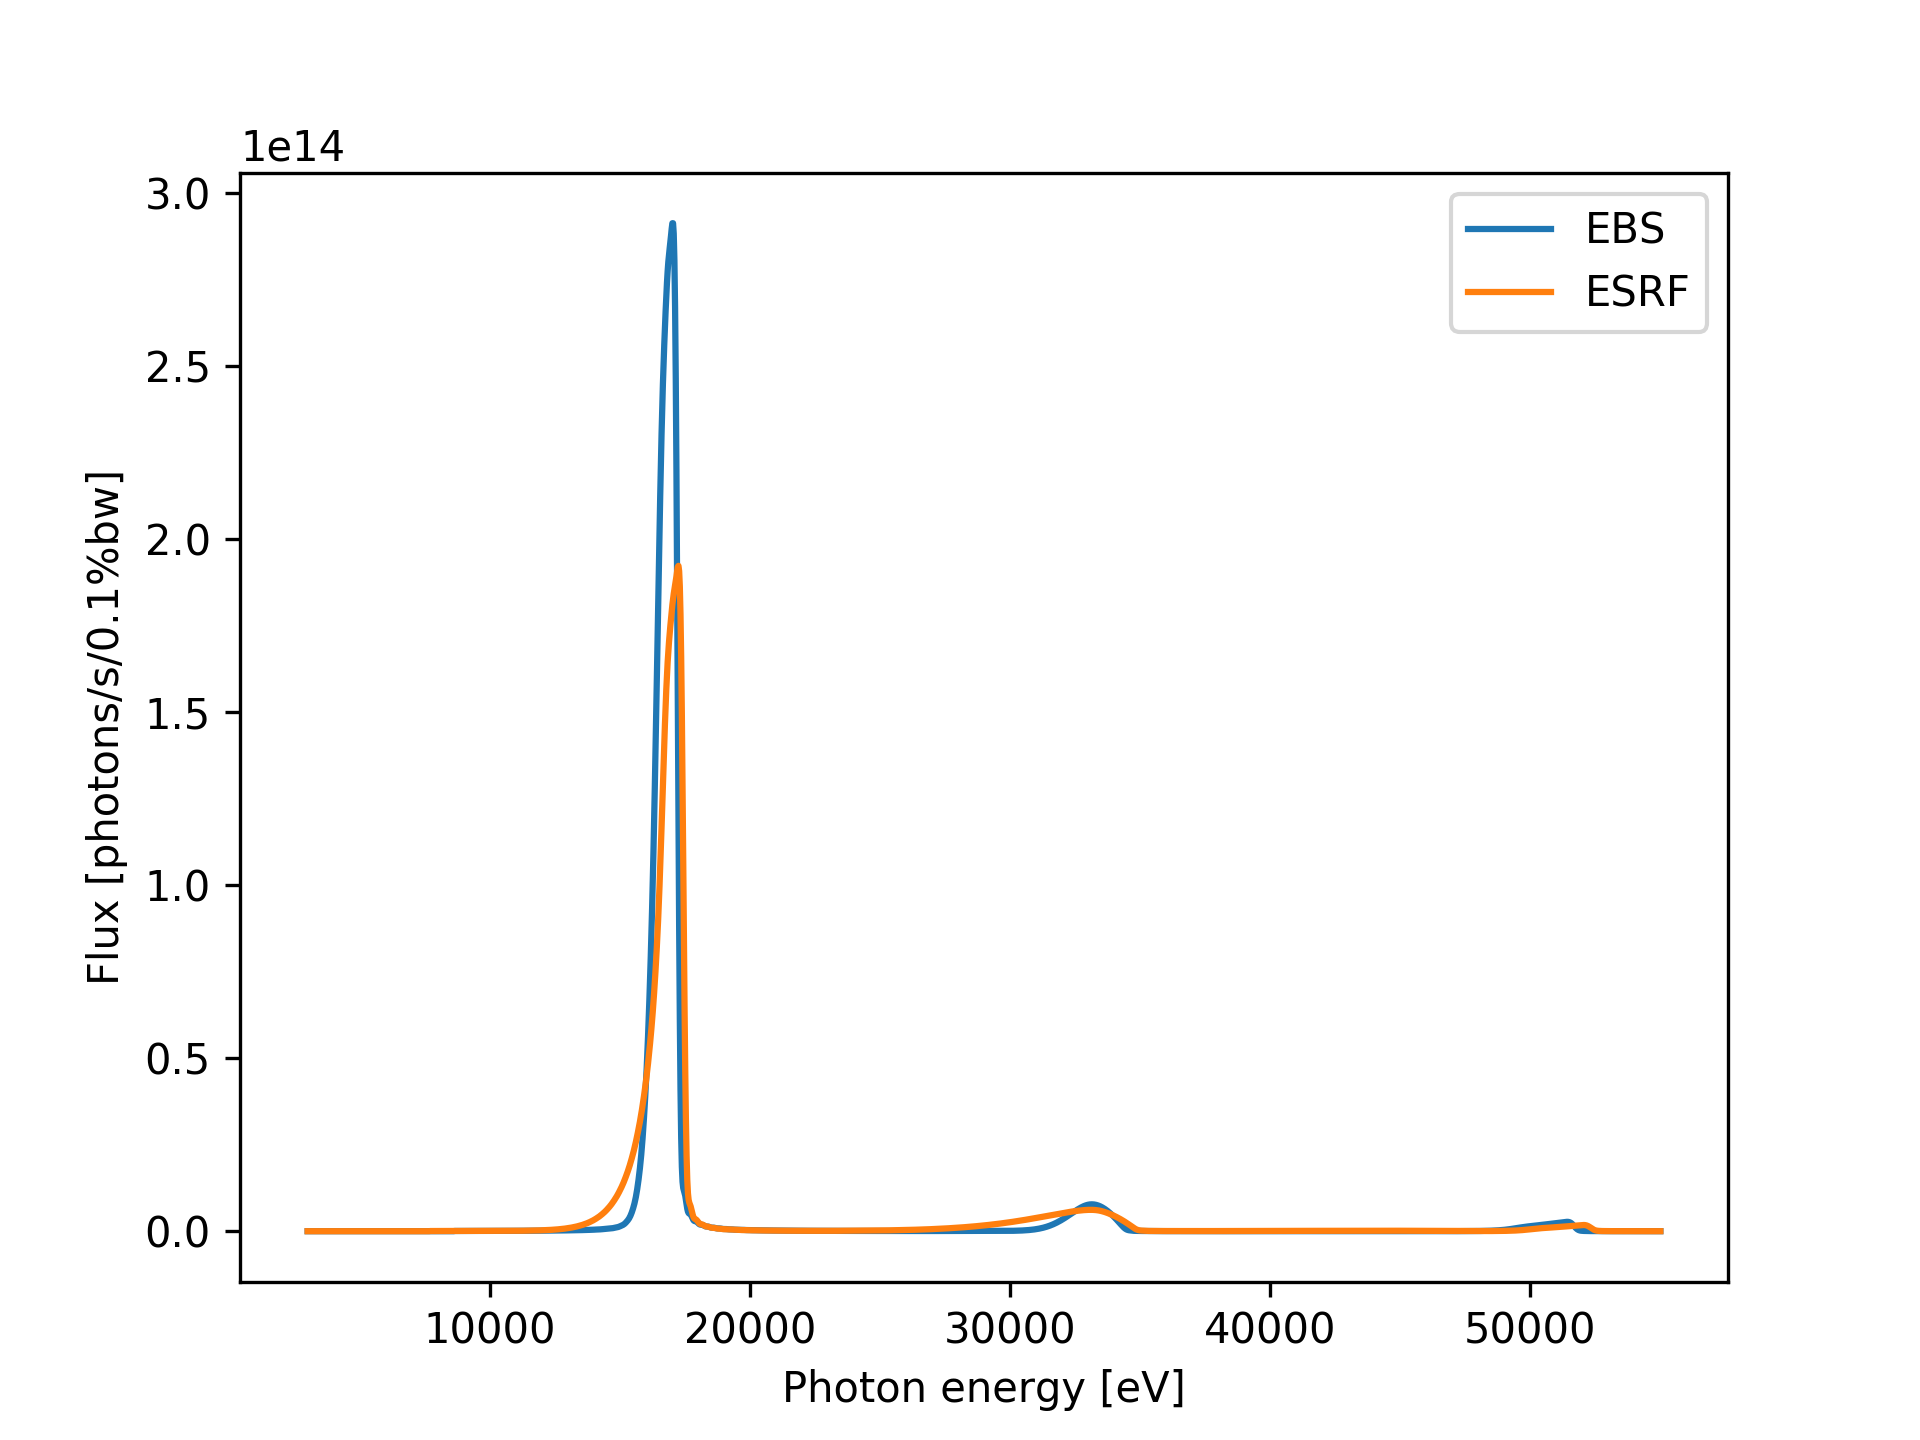
\includegraphics[width=0.8\textwidth]{GRAPHICS/fluxU18.png}
    \caption{Flux of the U18.3 undulator integrated over a square slit placed at 27.1~m from the ID centre with aperture of 1 and 4 mm.}
\end{figure}

Next we would like to estimate the geometrical transmitivity of the beamline, therefore we have to consider which optical element crop the beam and remove photons. This can be analysed using their angular acceptance or numerical aperture. The multilayer monochromator accepts the whole beam. We consider a VSS closed to $S_h=50~\mu$m in horizontal and fully opened in vertical. For ESRF its transmittivity is 1/8 (as discussed before) and 1 for EBS. In a similar way, the KB mirrors will crop the beam to a size that is the projection of their length to a direction perpendicular to the optical axis. Using mirror length of $L_v$=60 mm and $L_h$=26 mm for VFM and HFM, respectively, and incident angle of 15 mrad, the KB is behaving like an aperture of $900 \times 390 \mu m^2$. We get N.A. values of 6.2$\times$21.6 $mu$rad (aperture size divided by the distance from the mirror to the VSS in H and to the source in V). The transmittivity coefficient is the ratio of the accepted N.A. over the beam divergence, resulting 9.5\% (H) and 0.18\% (V)for ESRF and 16.3\% and 0.18\% for EBS. The overall transmission is the product of H and V ratios, therefore 0.2\% for ESRF and 2.95\% for EBS, therefore 3.8 $10^{11}$ photons/s for ESRF and 8.5 $10^{12}$ photons/s for EBS. 
\todo{check with references $10^9$ at 33.6 keV. I get: 1.6e+15 * 0.00295 * 0.7**3 = 1.62e+12. How closed are the slits? }

One can also discuss some simple consequences about the beam coherence. The coherence fraction (CF) \cite{arxivCF} of the undulator beam is the occupation of the lowest coherent mode, as it will be discussed in Section~\ref{level2}. An approximated estimation of it can be obtained using Eqs.~\ref{eq:photon small sigmas} and \ref{eq:photon big sigmas}. The CF in its the horizontal and vertical planes are
\begin{equation}\label{eq:coherent fraction}
 CF_{(h,v)} = \frac{\sigma_u \sigma'_u}{\Sigma_{(h,v)} \Sigma'_{(h,v)}},
\end{equation}
and the total coherent fraction is the product of both (CF=CF$_h \times $CF$_v$). An estimation of the CF calculated in such a mode give CF=0.12\% for the ESRF and 2.73\% for EBS at 17 keV photon energy. The CF roughly indicates the ratio of the ``coherent photons'' over the total number of photons. It is a good indicator of the quality of a coherent beam (a fully coherent beam has CF=1 and an incoherent beam CF=0). The beamline optics acts as a ``coherence filter'' by removing the ``bad'' or ``incoherent'' photons and in consequence increasing the CF. A complete cleaning is impossible because of the spatial overlapping of the different coherence modes. However, apertures centered at the optical axis would make the work. If we compare the values transmittivity of the beamline due to geometrical clipping  (0.2\% for ESRF and 2.95\% for EBS) with the the CF values, we remark that they are very close. This implies that the beam at the focal position would be highly coherent because the fraction of the photons removed from the beam matches the CF value that quantify the fraction of ``good'' or ``coherent'' photons. 

To assess the focused beam size, one can idealize the beamline in two parts. First, the ML monochromator and VSS that will prepare a coherent plane wave as the source is very far from the sample position. Second, the KB has a double role, acting as a focusing element of focal distance $f$=5 cm, but also crops the beam as as it would be done by a square aperture of $D \times D=$ 400$\times$400 $\mu m^2$ (the length of the mirror projected in a plane perpendicular to the beam propagation) \inred{(we obtained 900 in H, that will be reduced by 0.5 as propagated from 10 cm to 5 cm upstrem from the sample, and 390 in V approximated by 400)}. This aperture has two effects: i) as discussed before, it removes a lot of off-axis photons increasing the CF to a value close than one, and ii) make a broadening of the focal spot because of coherent diffraction. We know from optics that the diffraction by a square aperture of a collapsing spherical wavefront has an intensity distribution proportional to $\sinc^2(k D x/2 f) \sinc^2(k D y / 2 f)$, where $k=2\pi/\lambda$, and $x$ ($y$) is the horizontal (vertical) coordinate . Considering that the FWHM of $\sinc(x)$ is approximately 2.78, one obtains a FWHM of 7.75$\times$7.75 nm$^2$ for the focal spot. This spot size is of the order or larger than the one obtained by geometrical considerations, therefore contributing significantly to the size of the focused beam. One can conclude that for the conditions in use this is a diffraction limited beamline. 


In summary, we show in this section how simple analytical calculations that can be done in its major part ``by hand'' help to estimate the geometrical beam size at focal position (17$\times$5 nm$^2$ for ESRF, 10$\times$5 nm$^2$ for the EBS) the flux (3.8 $10^{11}$ photons/s for ESRF and 8.5 $10^{12}$ photons/s for EBS) and also anticipate that the beam is highly coherent producing a diffraction limited focal spot of  7.75$\times$7.75 nm$^2$. We ignored at this point the effect of real optics containing surface errors, the reflectivity of the elements, and other aspects that will be treated in depth in the next sections. This is, however, the first step to be done when analyzing a beamline. It also helps in having a critical eye or sanity check on the numerical calcuations that will provide more precised values, but must remain the this order of magnitude.  


 %-------------------------------------------------------------------------
 % Manuel
 %-------------------------------------------------------------------------
\subsection{Ray tracing calculations}
\label{level1}

In this section we perform ray tracing calculations to study the effect of real optics (including aberrations and slope errors) to the beam size and beamline transmittivity. The first subsection deals with the effect of aberrations and transmittivity due to geometrical considerations. The second subsection shows how the effect of slopes errors the KB mirrors degrade the focal spot.  

Ray tracing is a simulation method based on tracing some light rays along the optical system from the source to the image and retrieve the statistics of rays at the image to measure beam characteristics. For simple systems one can perform ray tracing even by hand, selecting some principal rays that will define the location and envelope of the image. Using computers one can trace thousands of rays and calculate the position and divergence distribution of the rays using statistics. Rays are usually generated by Monte Carlo sampling the source characteristics. Ray tracing is based on geometrical optics: a ray is a solution of the Helmholtz equation and travels in vacuum along straight line. Rays are intercepted by the optical elements, which change their trajectory. For reflectors, this change of direction is given by the specular reflection laws. For refractors, the change of direction os defined by the Snell law. Because Snell law uses the refraction index which is wavelength-dependent, it is then interetisting to add additional parameters to each ray, such as the wavelength. This will permit to calculate the refraction index that has to be used by each ray. The information of each ray can also be extended to include some intensity, or better electric field amplitude. This allows to extend the pure geometrical tracing to include physical models that take into account the optical element reflectivity or transmittivity. This combination of using a geometrical model plus a physical model allows to simulate every element used in a synchrotron beamline, such as mirrors and combination of them (e.g., KBs); lenses, compound refractive lenses and transfocators; gratings of any type and shape, crystal systems, etc. Ray tracing is a simple and extremely powerful technique for calculating the main characteristics of the photon beam (size, divergence, photon distribution) at every point of the beamline. Although very powerful commercial ray tracing packages are available in the market, they are not suitable for synchrotron simulations because they do not cover the particularities of X-ray devices and sources. For that purposes, several packages created in the synchrotron community and are available, like SHADOW \cite{codeSHADOW}, RAY \cite{codeRAY}, McXtrace \cite{codeMCXTRACE} or XRT \cite{codeXRT}. SHADOW is probably the one that is more used and cited. We use SHADOW and its interface ShadowOUI \cite{codeSHADOWOUI}, available as a module of the OASYS suite.


% When analyzing an optical system producing an extremely high demagnification of the source one can think in several limiting factors that could affect the focal sizes calculated by hand in Table~\ref{tab:HandCalculations}. 

% \inred{REMOVE!!
% One limiting factor is that the system under consideration is not an {\it imaging system} so an intensity distribution at the source (e.g., a Gaussian distribution) is not necessary imaged into a the same distribution (Gaussian). To test that, we implemented the beamline as three ideal lenses, each of them representing an optical element: ML, KBV and KBH. Ray tracing simulation show that, indeed, the demagnified image of a Gaussian source by ideal lenses shows a vertical distribution that is not Gaussian (see Fig.~\ref{fig:ray tracing ideal elements}a ). The FWHM is not close to what is expected theoretically because of the high numerical aperture. The finite acceptance of the optical surfaces and apertures makes possible a significant reduction of the aberrations. The price to pay is of course a large reduction of the intensity. Defining the multilayer and mirror acceptances as slits right before the ideal focusing elements, we obtain the image sizes shown in Fig.~\ref{fig:ray tracing ideal elements}b. Here, the image dimensions are importantly reduced in horizontal for the ESRF-High$\beta$ because of a great cut in beam dimensions due to the effect of the 50$\mu$m VSS slit and KB acceptance. It can also be seen the complete absence of the tails also due to the effect of beam cut by the apertures.
% }

We performed ray tracing using the elliptical reflectors with finite dimensions as focusing elements. The reflector shape is chosen to be elliptical as this is the theoretical shape producing a point-to-point focusing. For a first calculation  the elliptical elliptical reflectors are considered perfect, and have no slope errors. 
The results in Fig.~\ref{fig:ray tracing}a show two facts. One is that the migration from ESRF lattice to the EBS will significantly improve the horizontal size, and the VSS is not needed. For EBS, the whole beam passes though the VSS, producing a final spot with almost Gaussian horizontal intensity profile instead of the step distribution for ESRF. Secondly, one can observe a much larger luminosity in the EBS case. The transimittivity values are 0.165\% for ESRF and 2.28\% for EBS. These values confirm the analytical estimations (0.2\% for ESRF and and 2.95\% for EBS). As mentioned before, these values are similar to the coherent fraction \cite{coherentfraction} (0.12 for ESRF and 2.73\% for EBS), meaning that a very high coherence of the beam is expected, therefore some degradation of the beam by clipping the beam by apertures and element acceptance is expected. 

% Moreover, the treatment of the slope errors cannot be done without considerent effects of coherence, as discussed in \cite{hybrid}. This will be discussed in the next sections. 



\begin{figure}
\label{fig:ray tracing}
\centering
% \includegraphics[width=0.45\textwidth]{GRAPHICS/ideallensESRF.png}
% \includegraphics[width=0.45\textwidth]{GRAPHICS/ideallensEBS.png}
% 
% \includegraphics[width=0.45\textwidth]{GRAPHICS/ideallensaperturesESRF.png}
% \includegraphics[width=0.45\textwidth]{GRAPHICS/ideallensaperturesEBS.png}

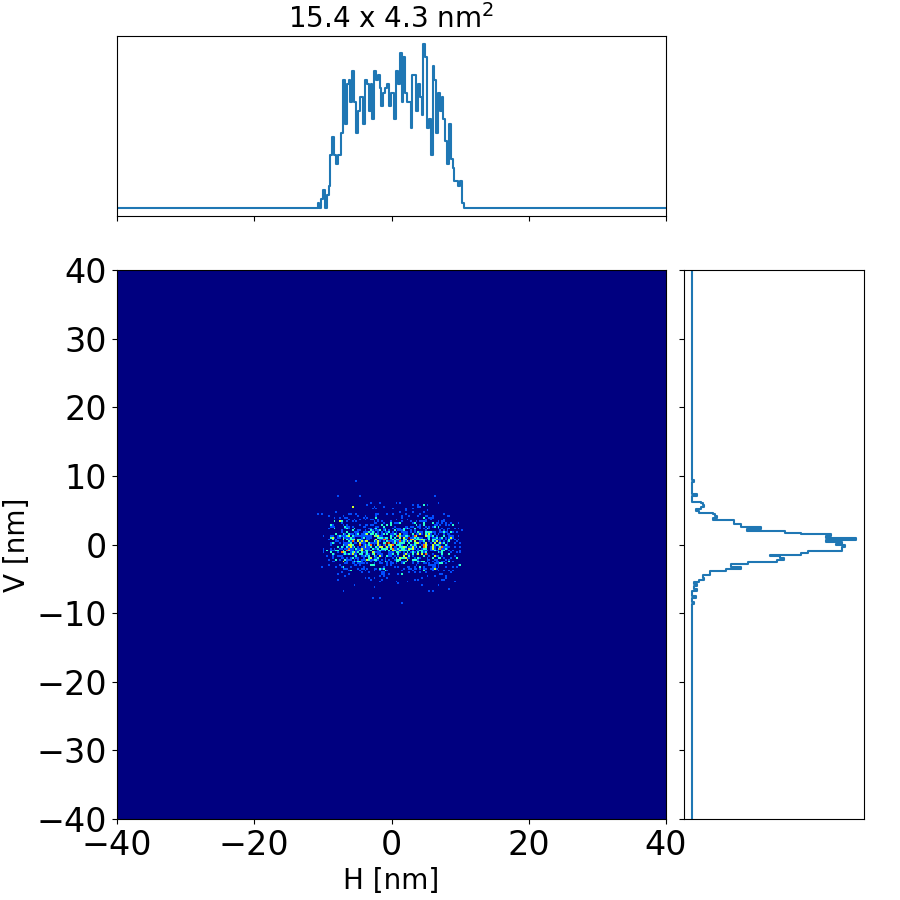
\includegraphics[width=0.45\textwidth]{GRAPHICS/idealelementsESRF.png}
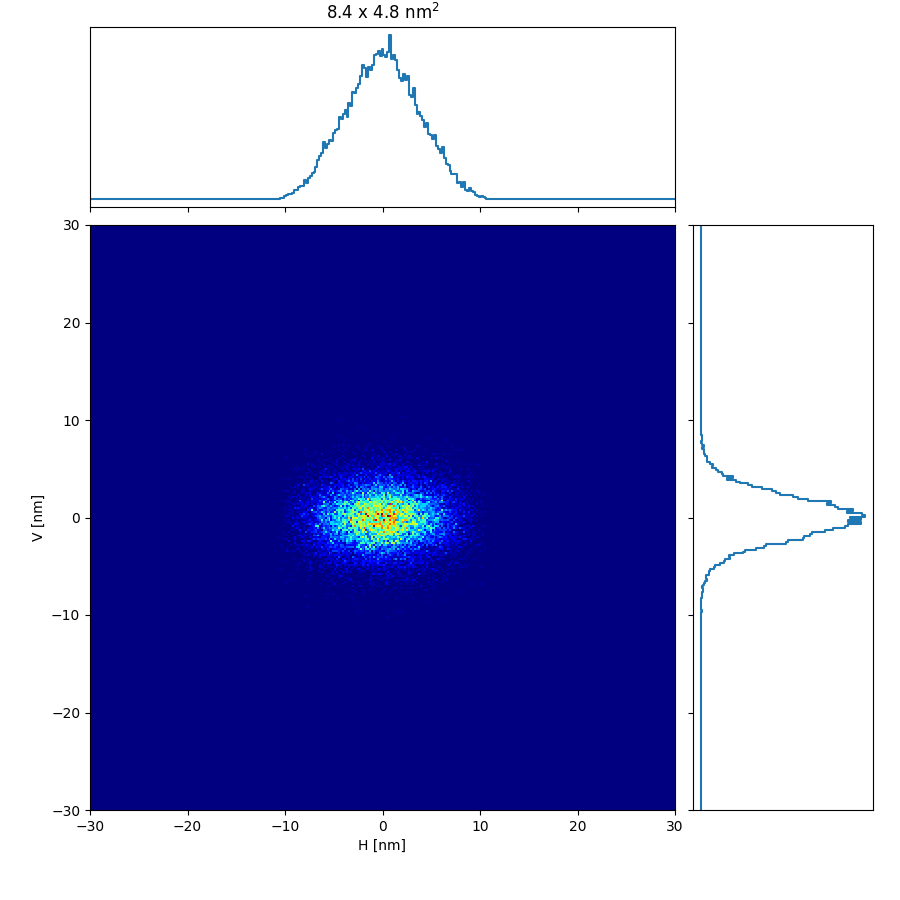
\includegraphics[width=0.45\textwidth]{GRAPHICS/idealelementsEBS.png}

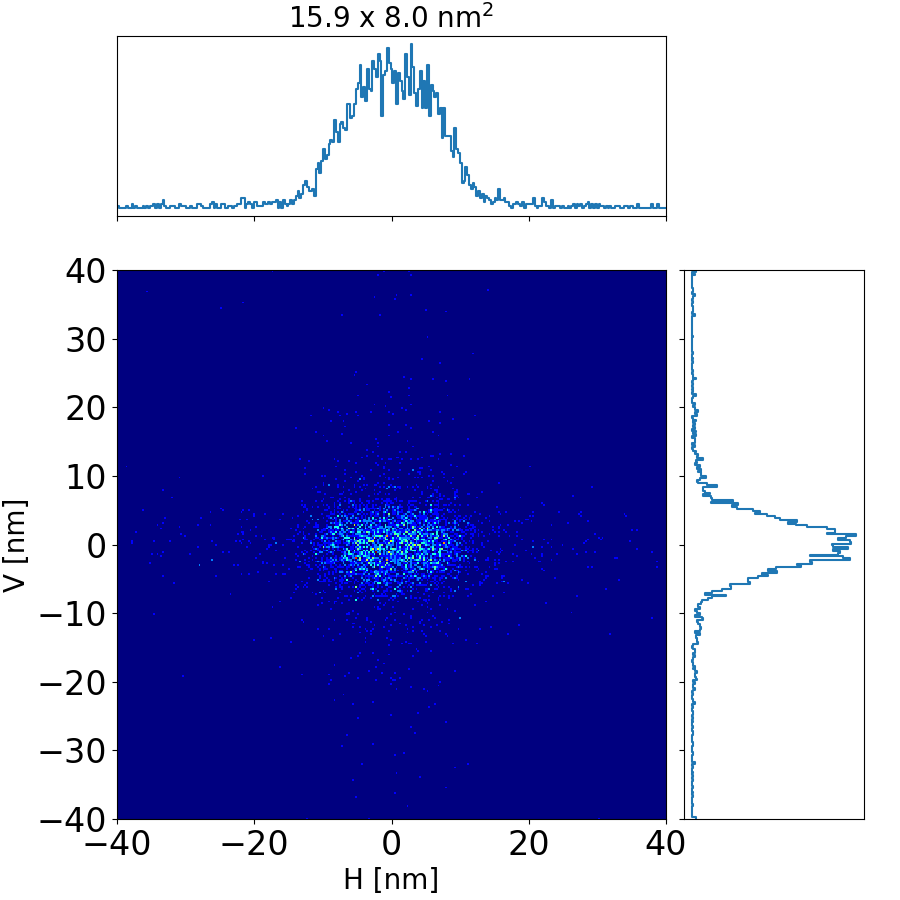
\includegraphics[width=0.45\textwidth]{GRAPHICS/hybridnoerrorsESRF.png}
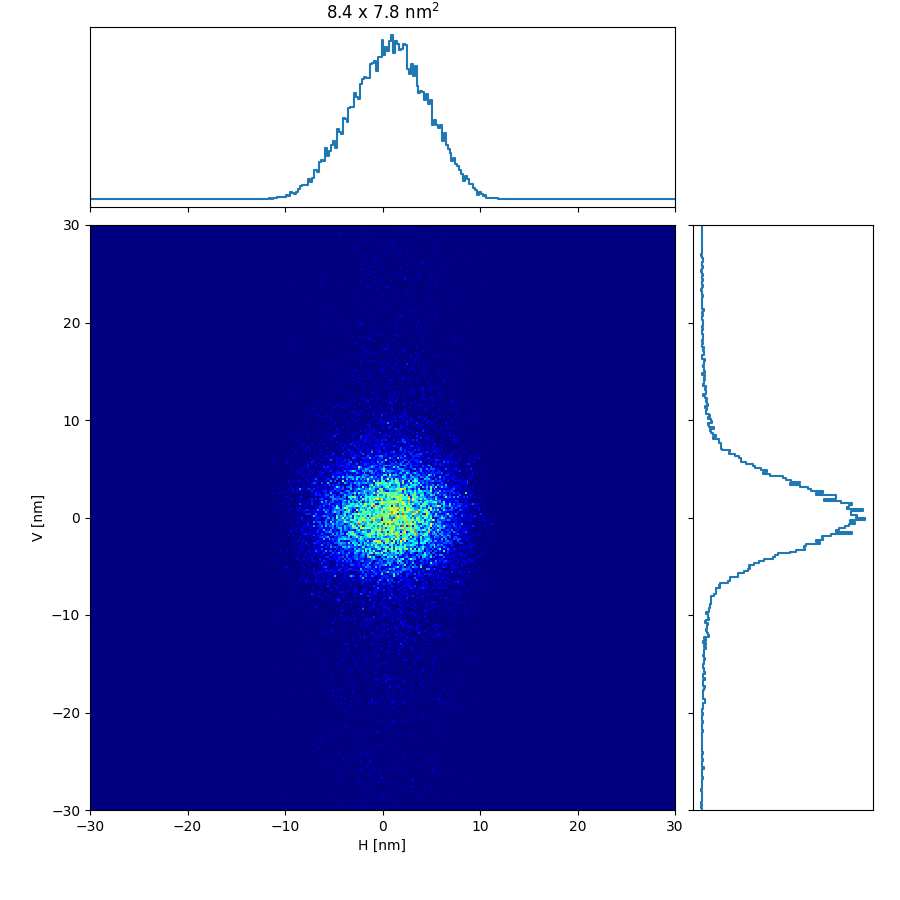
\includegraphics[width=0.45\textwidth]{GRAPHICS/hybridnoerrorsEBS.png}

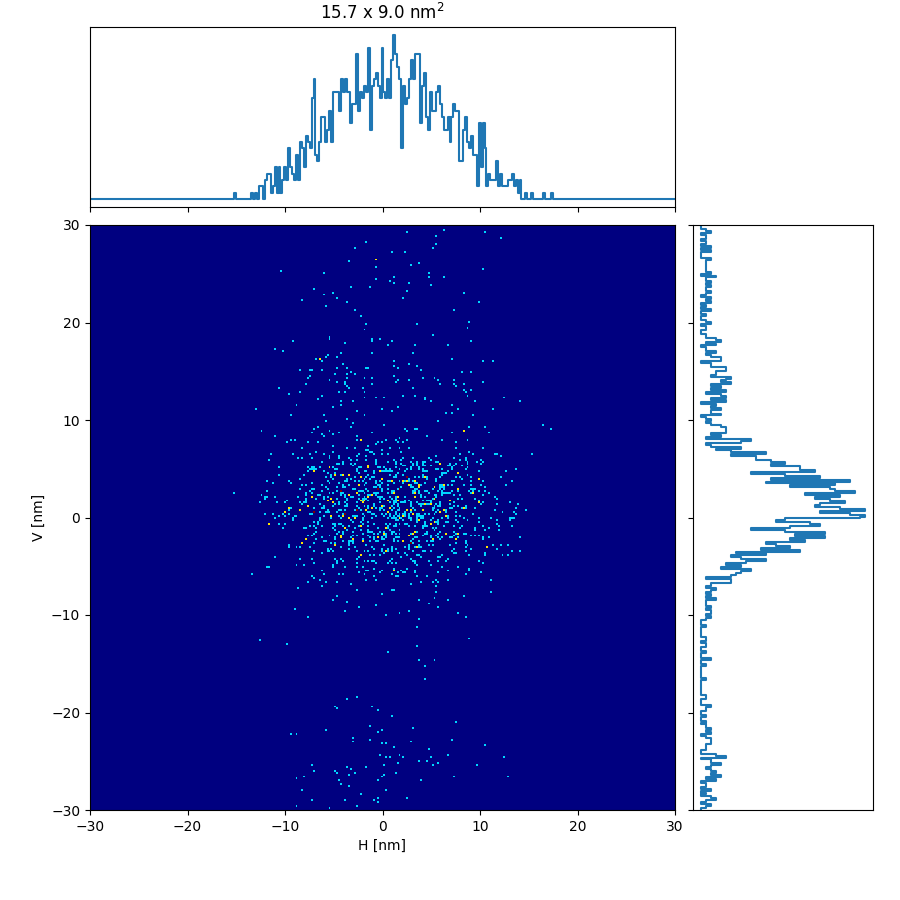
\includegraphics[width=0.45\textwidth]{GRAPHICS/hybriderrorsESRF.png}
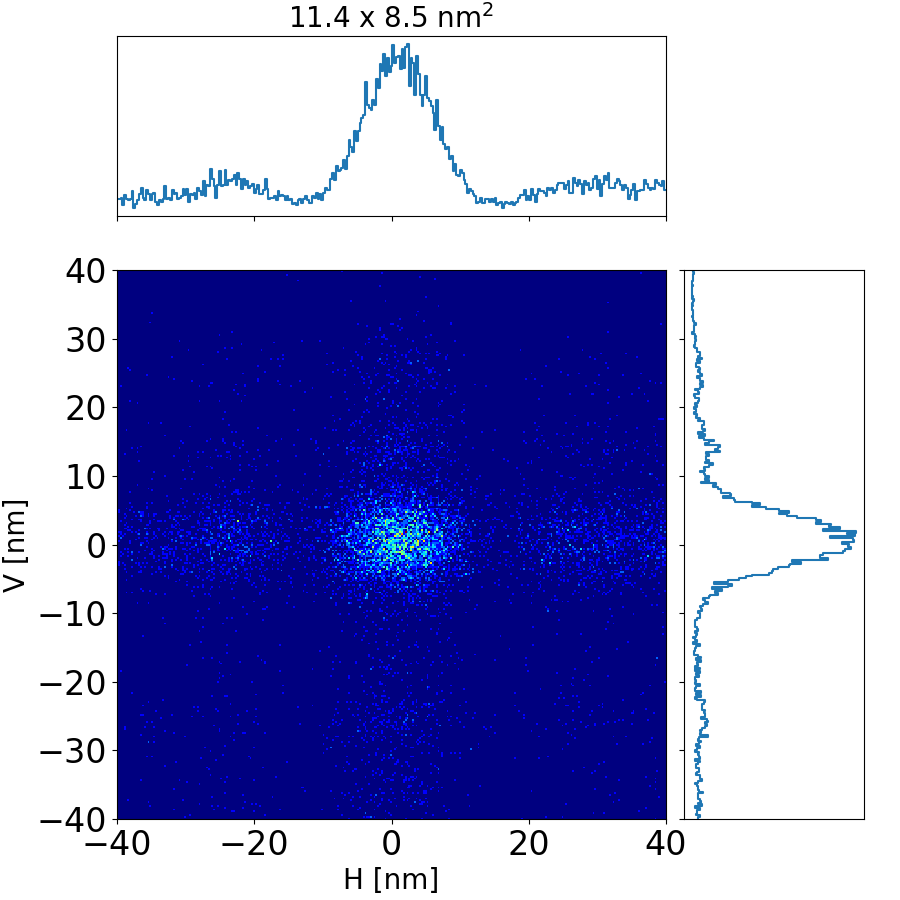
\includegraphics[width=0.45\textwidth]{GRAPHICS/hybriderrorsEBS.png}

\caption{Image produced by different types of ideal focusing for the ESRF (leftcolumn) and EBS (right column). The source with parameters in 
\ref{tab:HandCalculations}. 
The first row has been calculated using the elliptical reflectors (both for ML and KBs) but without slope errors. The focal beam dimensions are written in the plot title.
The second row shows the image calculated the hybrid option (ray tracing plus coherent diffraction) with elliptical reflecting surfaces. It shows the focal spot degradiation duw to the diffraction originated by cropping the beam by the KM mirrors. The calculation in the bottom row also include slope errors using the real mirror profiles measures at the ESRF metrology lab. It can be shown a further degradation and the growing of satellite structures in the vertical intensity distribution. 
}
\end{figure}


The HYBRID method \cite{hybrid} uses geometric ray tracing combined with wavefront propagation. The code computes diffraction effects when the beam is clipped by an aperture or by the finite size of the optics and can also simulate the effect of mirror figure errors when diffraction is present. The method can be applied to an entire beamline by simulating each optical element iteratively under the hypothesis of the validity of far field propagation in all intermediate propagations. If this is not the case, a near field version is available for investigating imaging by individual optics. The interest of the hybrid method is to assess in a fast way the influence of beam coherence because the code is considerably faster than the the full methods for dealing with the partial coherence of the synchrotron beam that are described below. Fig.~\ref{fig:ray tracing}b presents the results using the hybrid model for the beamline with ideal elliptical optical surfaces. When compared with the pure ray tracing in Fig.~\ref{fig:ray tracing}a it can be appreciated that the spot is broadened. This is more evident in the vertical direction, because the smaller focal size. The spot size is about 7-8 nm in V for both storage ring lattices, and in horizontal is about 15$\mu$m for ESRF-High$\beta$ and 11 nm for EBS. It is interesting to note the almost round spot that will be obtained with the new EBS lattice. 

The surface finish of the optical elements is another limiting effect for determining the size and intensity of the beam at the image position. It is possible to infere the effect of mirror imperfections and in particular slope errors by only knowing some statistical parameters such as the slope error Root Mean Square (RMS) and then building synthetic surface profiles to be used in the simulations. This is the typical mode to operate when designing a new beamline where the mirrors do not exist yet. However, in our case the mirrors already exist and have been extensively characterize at the ESRF metrology laboratory. It is therefore highly recommended to use metrology data from real mirrors, when possible. When not available, one can use data from existing mirrors from a database (e.g., \cite{dabam}) and extrapolate some of the effects to the hypothetical new mirrors. The metrology data of the mirrors for the beamline under study are presented in \todo{Appendix 1}. These experimental data are used in all the simulations in this paper. Simulations using the hybrid model including slopes errors are shown in Fig.~\ref{fig:ray tracing}c. It can be observed a small broadening of the peak due to slope errors, but, more importantly, a new satellite structure close to the vertical intensity peak is produced by the slope errors. 

\todo{
\begin{itemize}
 \item play with slope errors and use synthetic profiles to show the importance of the low frequencies in the intensity distribution?
 \item explain why KB errors are treated with hybrid and not with shadow. In Discussion section? 
\end{itemize}
}


 %-------------------------------------------------------------------------
 % Rafael
 %-------------------------------------------------------------------------

\subsection{Wave optics simulations}
\label{level2}

In this section the coherence properties of the beamline are analysed using, again, different methodologies classified by complexity and computer resources. We first analyze the beamline supposing a fully coherent beam. Subection~\ref{wofry} shows a very simpified 1D model. Subsection~\ref{srw_se} used a full 2D model with accurate simulation of the undulator emission but without considering storage ring emittance. These simplifications permit to address diffraction effects by apertures and slope errors. Then we introduce methods to treat the partial coherence originated by the storage ring emittance. Two variants are shown, a Monte Carlo approach (subsection~\ref{srw_me}) that permits us to calculate in great detail the intensity dostribution of the focused beam, and a decomposition of the radiation in coherent modes (subsection~\ref{comsyl}) that allows to evaluate quantitatively the quality of the coherent beam.  


\subsubsection{Simplified wave optics simulation (coherent case in 1D with point source and ideal elements)}
\label{wofry}

The very long distance source-sample combined with a small source (in particular for EBS) makes this beamline suitable for experimental techniques requiring a highly coherent beam. Indeed, it has been shown that the clipping of the beam, mainly due to the acceptance of the KB mirrors produces a significant broadening of the focal spot.  As discussed in Section~\ref{level0}, very simple calculation of the diffraction limit can be sone using a convergent spherical beam clipped by a slit of 400$\times$400$ \mu$m$^2$ placed at 5cm upstream the focus (at the second KB mirror position). The slit vertical size corresponds roughly to the horizontal acceptance of the seconf KB mirror, and it is approximately the same in vertical. A simple simulation of diffraction by a square slit using OASYS is shown in Fig.~\ref{wofry400um}. It reveals a spot of less than 10 nm, thus confirming the analytical predictions, and qualifying this beamline to be a diffraction limited beamline.  

\begin{figure}
\label{wofry400um}
\centering
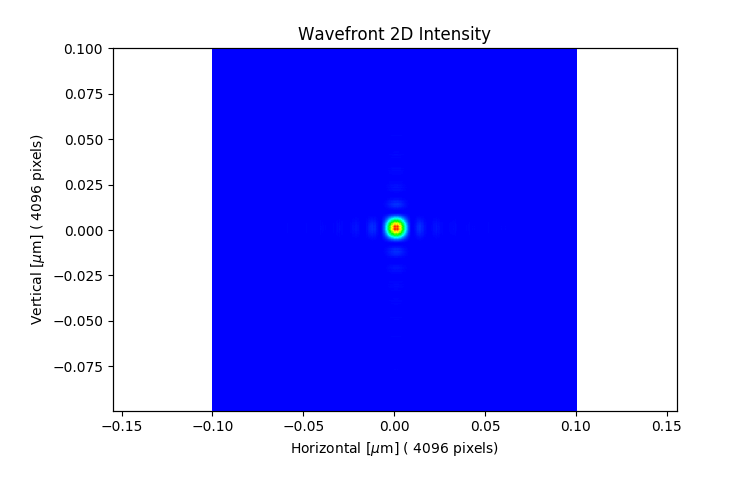
\includegraphics[width=0.45\textwidth]{GRAPHICS/wofry400umslit.png}
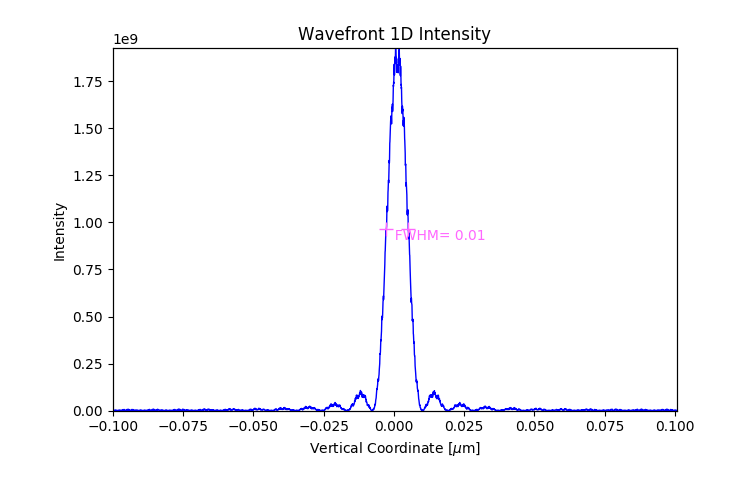
\includegraphics[width=0.45\textwidth]{GRAPHICS/wofry400umprofile.png}
\caption{Diffraction spot producedof a spherical wavefront (R=-50mm) by a 400x}
\end{figure}

We perform here a simplified wavefront simulation in 1D, thus separating the simulations of the horizontal and vertical planes. The source can be simplified by using a point source (spherical wavefront) and applying a Gaussian intensity profile with $\sigma=\sigma'_u d$ with $\sigma'_u$ given by Eq.~\ref{eq:photon small sigmas} and $d$ the distance from the point source to the observation plane. Each optical element can be simplified by separating its action in two parts: the focusing behaviour implemented as an ideal lens, and the finite size because of the boundaries, implemented as a slit. The WOFRY package in OASYS permits to do this work, and it is possible to arrive to a satisfactory result in a few iterations. The beam size at different positions of the beamline are shown in Table~\ref{tablewofry1D}. The final image profiles are in Fig.~\ref{wofry1D}.

\begin{table}[]
    \centering
    \caption{Beam sizes calculated with simplified wave optics propagation (point source and ideal lenses with aperture for modeling the element dimensions). 
    }
    \label{tablewofry1D}
    \resizebox{\textwidth}{!}{%
    \begin{tabular}{cccccc} 
    % using WAVEOPTICS WOFRY workspace
    Element:                & ML            & VSS          & KBv               & KBh           & sample        \\
    Position [m]:           & 28.3          & 40.00        & 184.90            & 184.95        & 185.00        \\
    H beam size [$\mu$m]:   & 329           & 1.11         & 4084              & 390           & 0.008         \\
    V beam size [$\mu$m]:   & 329           & 466          & 899               & 450           & 0.007         \\ 
    H scaling factor:       & 1.0           & 0.01         & 440               & 1             & 0.00002       \\
    V scaling factor:       & 1.0           & 0.64         & 5                 & 0.5           & 0.00002       \\
    \end{tabular}%
    }
\end{table}

\begin{figure}
\label{wofry1D}
\centering
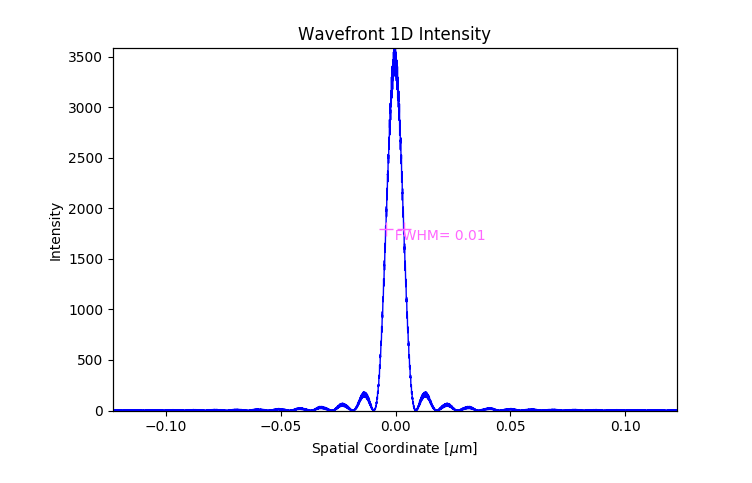
\includegraphics[width=0.45\textwidth]{GRAPHICS/wofry1Dh.png}
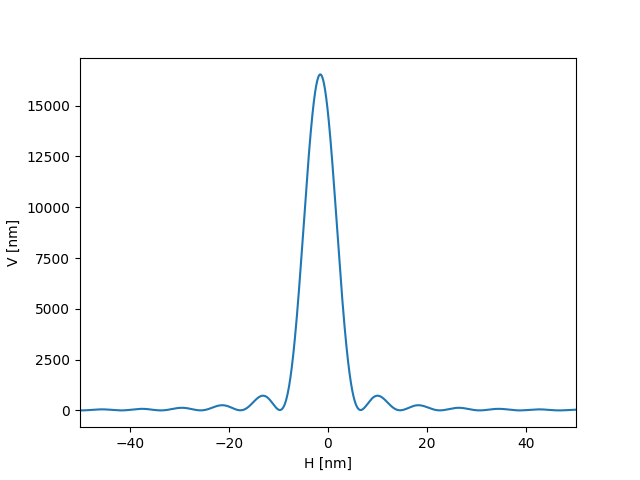
\includegraphics[width=0.45\textwidth]{GRAPHICS/wofry1Dv.png}
\caption{Intensity distribution at the focal position in horizontal plane (left, FWHM=8.1 nm) and in vertical plane (right, FWHM=7.1 nm).
\todo{implement a sort of multielectron system - implement the slope error. In Discussion? } 
}
\end{figure}


\subsubsection{Full wave optics simulation for coherent case}
\label{srw_se}
% The reduction on the electron beam emittance, by reducing the electron beam horizontal size, leads to an increase on the horizontal lateral coherence of the radiation emitted by an undulator in the symmetry point of a straight section \cite{paper}. Incoherent simulation methods may be insufficient for a full assessment of the beamline design. To accurately account for coherence effects, one has to resort to wave optics simulations (commonly referred to as wave propagation).
% 
A next step in the wave optics simulation is, maintaining the full coherence, to generate a 2D source wavefront that matches in detail the real source (an undulator in a storage ring) and then simulate the propagation of such a wavefront through the optical elements with models that match well the characteristics of the real elements. The source simulated is the on-axis-single-electron emission from the U18.3 undulator tuned to its first harmonic at $E=17225$ eV. The emission by a single-electron is fully coherent. Once the source is defined, one has to go around on how to simulate the beamline optical elements. Increasing the complexity of the simulations one can: a) use ideal thin lenses preceded by slits to emulate finite aperture (as done in the 1D model presented in Section~\ref{wofry}); or b) use grazing incidence focusing optics models \cite{Canestrari2014}. On the top of that, one can add the effect of imperfect optics to the simulations, i.e. slope errors. 

The computer code chosen for these calculations is Synchrotron Radiation Workshop (\textsc{srw}) \cite{codeSRW}, which over the past two decades has been extensively benchmarked throughout different synchrotron radiation facilities and has become widely accepted within the X-ray community.

Figure \ref{fig:SingleElectron} shows the horizontal integrated intensity at the focal position for the ID16A. It can been seen that there is little difference between using thin ideal lenses or the elliptical mirror model. The elliptical mirror presents a slight reduction in intensity and asymmetry but no significant difference is found, which is in accordance with what is reported in \cite{Canestrari2014}. Notice that the differences are minimal and to remark them we have chosen log plots to represent the intensity distributions at the focal position. It is also important to mention that this equivalency between ideal lenses and elliptical mirrors is only valid at the focal position vicinity: down- or upstream the focal position, differences are not negligible \cite{Canestrari2014}. 

It is also possible to add slope errors to the simulations to study the degradation on the focal spot quality (Fig.~\ref{fig:SingleElectron}). For that, the available available metrology data \inred{(Appendix 1)} are used. For both cases (i.e., simulating the beamline using thin optical elements or elliptical mirrors), the beam sizes calculated as the FWHM at the focal position are little affected by the presence of the slope errors (see Table \ref{tab:SRW_results}). There is a significant reduction and shuffling of the interference fringes observed with no slope error. They are almost cancelled, with is an important raise of the background level: the radiation found on the main lobe (focus) shifts to the side lobes when the slope errors are considered. This is accompanied by an obvious reduction on the peak intensity. Table \ref{tab:SRW_results} compiles the beam sizes at focal position for mentioned simulations.

\begin{figure}
    \centering
        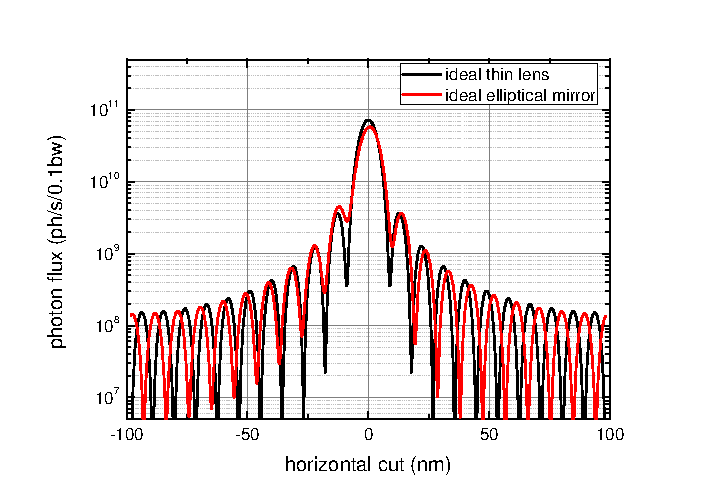
\includegraphics[width=4.25cm]{GRAPHICS/se_idealTE_idealOE_h.pdf}
        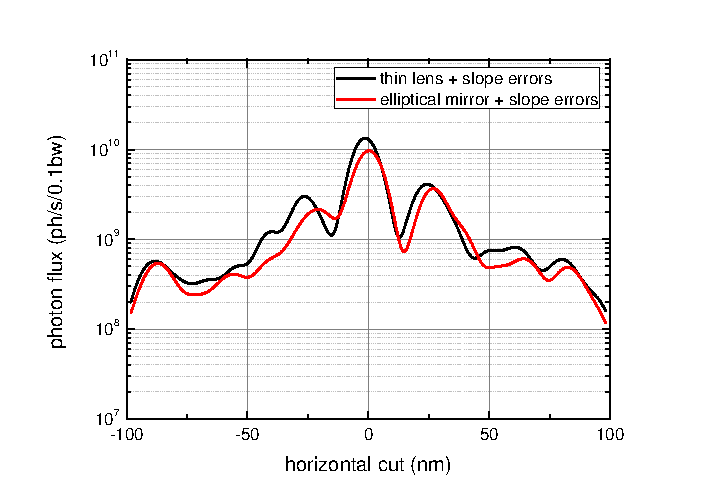
\includegraphics[width=4.25cm]{GRAPHICS/ebs_slopeTE_slopeOE_h.pdf}
    \label{fig:SingleElectron}
    \caption{Wavefront propagation from a single electron emission through the ID16A beamline. Left: the perfect focusing with ideal lenses (black) is compared with the focusing using elliptical mirrors (red). Right: the same as in the previous plot, but adding the effect of the mirrors slope errors in bothe cases.}
    %Simulations took less than one minute in a desktop computer Intel Core i7 with 8Gb of RAM memory.}
\end{figure}


\begin{table}\label{tab:SRW_results}
\centering
\caption{Beam dimensions (FWHM) at the focal position for different models of focusing elements.}
\resizebox{\textwidth}{!}{%
\begin{tabular}{ccccc}
Focusing elements                 & Plane      &  Single electron & EBS         & ESRF       \\
ideal lenses/ elliptical mirrors  & Horizontal &  7.94/7.97       & 12.20/12.70 & 17.50/16.80 \\
the same, with errors             & Horizontal &  9.35/10.50       & 12.90/13.65 & 17.70/17.03 \\
ideal lenses/ elliptical mirrors  & Vertical   &  7.11/7.26       & 8.40/9.02   & 8.24/8.77    \\
the same, with errors             & Vertical   &  7.44/8.46       & 8.66/9.87   & 8.52/9.66    \\                                                                 
\end{tabular}
}
\end{table}


\subsubsection{Full wave optics simulation: partial coherent case by means of multielectron Monta Carlo sampling}
\label{srw_me}
The wavefront propagation methodology is based in the sampling of a single wavefront (monochromatic and coherent) in a 2D space (in horizontal and vertical spatial dimensions) at a given point of the beamline. This initial point considered as source cannot be the source physical position, because i) when condidering point or spherical waves all the intensity would come in a single pixel so the wavefront is ill-defined, ii) when using synchrotron sources (i.e., undulators) theory \cite{jackson} permits the calculation of the radiation in positions far from the electron trajectory. The limitation of the method is that one wavefront is not representative for a beam that, in storage rings, is produced by the emission of many electrons circulating through the corresponding magnet structure. Diffraction limited sources would emit radiation that can be described in good approximation by a single wavefront. But even for new ultra low-emittance storage rings (improperly called diffraction-limited sources, see discussion in \cite{coherentfraction}) the contribution of the electron dimensions ($\sigma_{e(h,v)}$ and $\sigma'_{e(h,v)}$) is not negligeable as compared with the natural emission of radiation ($\sigma_u$ and $\sigma'_u$ for undulators as in Eq.~\ref{eq:photon small sigmas}). To account for this effect one should complete or extend the wavefront simulations to take into account that in fact not only a single wavefront contributes to the properties of the beam. There are three approaches currently used: 1) use of convolutions, 2) Monte Carlo multi-electron sampling, and 3) Propagation of coherent modes. The convolution method consist in calculating the emission characteristics and then convolve the resulting intensity with Gaussians describing the electron beam. This method is simple and fast, as only requires simulation of a single wavefront. However, it presents two important limitations: i) it can only be applied to the intensity calculations and not to other parameters of interest for describing coherence, such as degree of coherence, etc., and ii) it can be applied only at the source position: it is usually unknown how the different optical elements will affect the source contribution to the phase space. The next method, the Monte Carlo multi-electron propagation, it is an statistical method based on the idea that one can exactly calculate the emission and its propagation for one electron that is deterministically described by its initial conditions at the entrance of the magnetic structure. It is therefore possible to perform many simulations for different initial conditions of the travelling electron and make the propagation along the beamline until the observation plane. Then one can statistically combine the different wavefronts (one for each electron) to obtain a sampling of the intensity and other magnitudes useful to describe partially coherent beams. This method presents two difficulties. One is convergence. One cannot know a priori how many electrons must be sampled to obtain a given level of accuracy. The second is computing resources. The emission of each electron must be calculated at the source level, propagated along every element of the beamline, and the resulting wavefront must be analyzed to extract the information to be scored and stored. The third method, the propagation of coherent modes wil be discussed in the next section. 

The Monte Carlo multielectron method has been proposed by O. Chubar and it is fully implemented in SRW \cite{codeSRW}. We have used this code for the calculations presented in this section.  

\begin{figure}
    \centering
        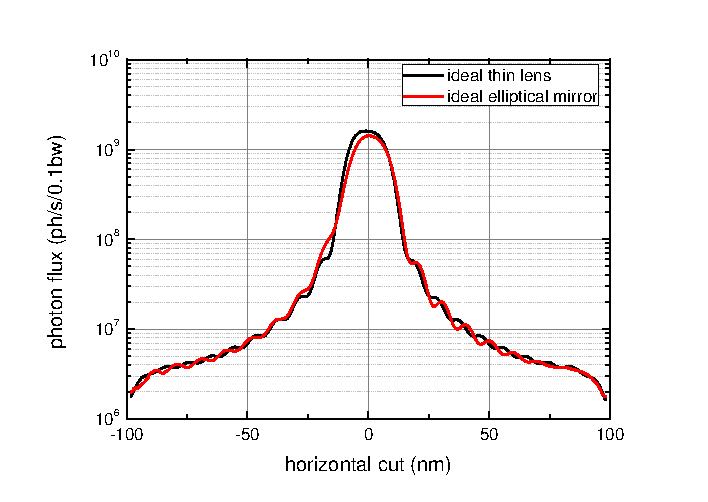
\includegraphics[width=4.25cm]{GRAPHICS/esrf_idealTE_idealOE_h.pdf}
        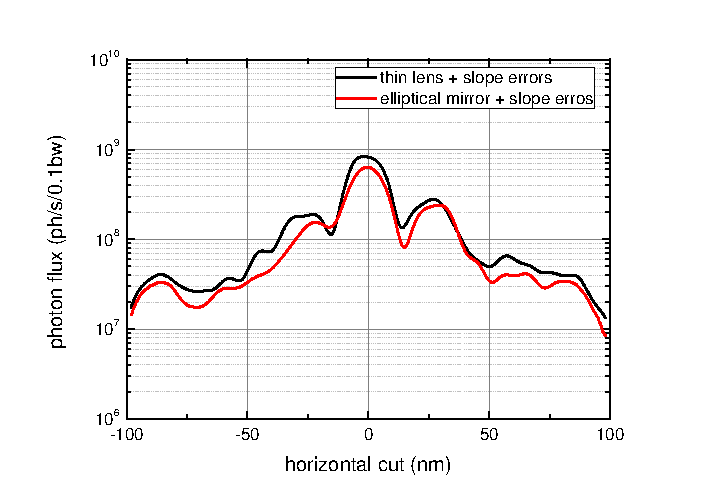
\includegraphics[width=4.25cm]{GRAPHICS/esrf_slopeTE_slopeOE_h.pdf}
    \label{fig:FiniteEmittanceA}
    \caption{Wavefront propagation from the ESRF magnetic lattice through the ID16A beamline.}
\end{figure}

\begin{figure}
    \centering
        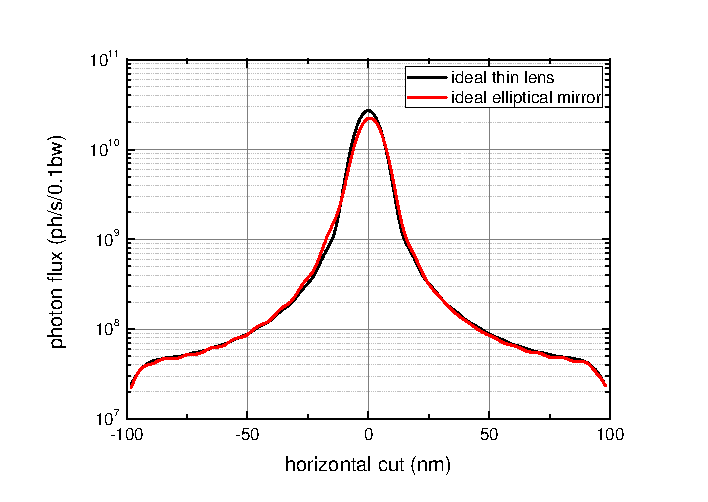
\includegraphics[width=4.25cm]{GRAPHICS/ebs_idealTE_idealOE_h.pdf}
        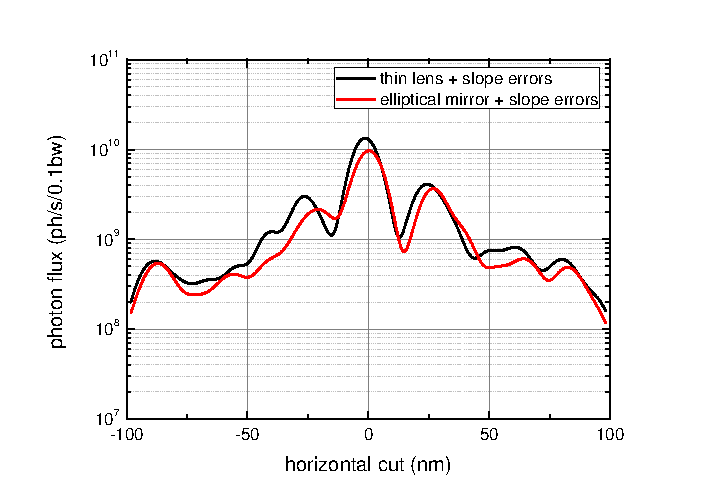
\includegraphics[width=4.25cm]{GRAPHICS/ebs_slopeTE_slopeOE_h.pdf}
    \label{fig:FiniteEmittanceB}
    \caption{Wavefront propagation from the EBS magnetic lattice through the ID16A beamline.}
\end{figure}


The source used for simulations is the U18.3 undulator tuned to its first harmonic at $E=17225$ eV with a finite emittance electron beam (see Table \ref{tab:eBeam}). Two set of parameters were used for the electron beam: the current machine parameters at the ESRF (high-$\beta$) and the EBS straight sections (Tables \ref{tab:TableSources} and \ref{tab:eBeam}). 

Simulations for both storage ring lattices were carried out modelling the beamline using thin ideal lenses and elliptical mirror models with and without the addition of the slope errors. Results are presented in Figures \ref{fig:FiniteEmittanceA} and \ref{fig:FiniteEmittanceB}; and Table \ref{tab:SRW_results}.

The same observations made on the previous section (full coherent simulations) are pertinent here: there is a reduction on peak intensity when comparing single lens model with the elliptical mirror. The beam sizes and shapes are similar at the focal position, only.

% 
% Synchrotron radiation on the hard X-rays regime is hardly full coherent even for the so-called diffraction limited sources (see Table \ref{tab:Coherence}). To better describe the nature of the emitted radiation, one makes use of the partial coherent simulations using the \textsc{srw}, i.e. incoherent addition of the intensity from the emission from electrons sampled from the source's 6D phase-space \cite{Chubar2011b}. This is a natural extension from the method presented on the previous section.


% 
% \newpage
% 
%  %-------------------------------------------------------------------------
%  % Manuel (?)
%  %-------------------------------------------------------------------------
%  
\subsubsection{Full Wave optics simulation: partial coherence case by means of coherent mode decomposition}
\label{comsyl}
% 
% One of the mentioned drawbacks of the Monte Carlo multielectron methods is the a-priori unability to determine the size of sampling space (i.e., how many electrons) for accurate calculations. 
% Another important limitation is the impossibility with available computer resources to store (although can be computed) the full 4D matrices fully describing the partial coherence properties (cross spectral density) at any point of the beamline. 

The cross spectral density (CSD) (sometimes called mutual intensity) completely describes the coherence of a beam. 
At a given plane at a distance $z$ from the source, for a photon beam of frequency $\omega$, the CSD is the correlation of the radiated electric fields between two spatial points $(x_1,y_1)$ and $(x_2,y_2)$:

\begin{equation}\label{CSD}
W(x_1,y_1,x_2,y_2;z,\omega) = <E*(x_1,y_1; z,\omega) E(x_2,y_2;z,\omega)>
\end{equation}
where $E$ is the amplitude of the electric field, and $<>$ stands for the ensemble average. The CSD is at the origin of any other information about the coherence of the beam, like the spectral density $S$ (or, spatial distribution of the intensity): 
\begin{equation}\label{SD}
S(x,y,;z,\omega) = W(x,y,x,y,;z,\omega)
\end{equation}
or the spectral degree of coherence $\mu$:
\begin{equation}\label{SDC}
\mu(x_1,y_1,x_2,y_2;z,\omega) = \frac{W(x_1,y_1,x_2,y_2;z,\omega)}{\sqrt{ S(x_1,y_1;z,\omega) S(x_3,y_2;z,\omega}}
\end{equation}
that measures the coherence of the beam, from fully incoherent ($\mu=0$) to fully coherent ($\mu$=1). 
Eq.~\ref{CSD} can in principle be calculated using the Kim's convolution theorem \cite{kim1986} (see \cite{geloni2008} for a full discussion on the validity) but its storage is prohibitif in present computers: supposing sampling one spatial dimension by $N\approx1000$ pixels, a wavefront will contain $N^2$ pizels, and the CSD will be sampled over $N^4$ points. They are complex numbers (16 bits) so the only stockage is of the order of GB or TB. Considering also that the progagation of $W$ from a beamline position $z_1$ to another position $z_2$ will need 10$^8$ to 10$^{12}$ 4D integrals, one can easily imagine the physical impossibility to perform such calculations. 

A solution to this problem is the expansion of the CSD in coherent modes \cite{mandel_wolf}:  
\begin{equation}\label{decomposition}
 W(x_1,y_1,x_2,y_2;z,\omega) = \sum\limits_{m=0}^{\infty} \lambda_m \Phi_m^{*}(x_1,y_1;z,\omega) \Phi_m(x_2,y_2;z,\omega)
 \end{equation}
where $\lambda_m$ are the eigenvalues or weights, and $\Phi_m$ are the eigenfunctions or (orthonormal) coherent modes. 

A theoretical study and a numerical algorithm for the coherent mode decomposition of undulator emission in storage rings has been recently proposed  \cite{GlassThesis,GlassEPL} and is implemented in the computer package COMSYL \cite{codeCOMSYL}. The innovative concept is the numerical description of the undulator CSD in terms of its coherent modes $\Phi_m(x,y;z,\omega)$ and eigenvalues $\lambda_m $. One can define the mode distribution as
\begin{equation}
 d_m = \frac{\lambda_m}{\sum\limits_{i=0}^{\infty} \lambda_i},
\end{equation}
or the cumulated mode distribution like
\begin{equation}
 c_m = \sum\limits_{i=0}^{m} d_i.
\end{equation}
An important property of the coherent mode decomposition is that it optimizes the representation of the CSD when the series is truncated. In other words, truncating the series in Eq.~\ref{decomposition} up to the term $m$, the CSD obtained approximates better the exact CSD (this with infinite terms) than any other expansion. It also imply that the first term is more important than the second, and so on. The first or lower term (index zero) is the most important coherent mode. It permits to define the coherent fraction (CF) as the occupation of the lower coherent mode: CF=$d_0$. Obviously, a pretty coherent source will require less modes than a mostly incoherent source to arrive up to a certain representation of the CSD.

We performed COMSYL calculations for the U18.3 undulator radiation of ID16A of 1.4 m length using both the EBS and ESRF-High$\beta$ lattices. The obtained CF are 2.8\% for EBS and 0.13\% for ESRF-High$\beta$, indicating that the overall coherent flux emitted by EBS will be about 20 times the existing coherent flux with ESRF-High$\beta$. Fig.~\ref{fig:histomodes}a shows the cumulated occupation of the coherent modes for the full central cone undulator emission. It shows that the EBS cumulated occupation grows very steply with the number of coherent modes, whereas for ESRF the number of coherent modes needed to attain a given value of cumulated occupation much higher. This can also be shown in Fig.\ref{fig:histomodes}b, where the number of modes to fill 50\%, 75\% and 95\% of spectral density are compared for EBS and ESRF.   

\begin{figure}\label{fig:histomodes}
    \centering
        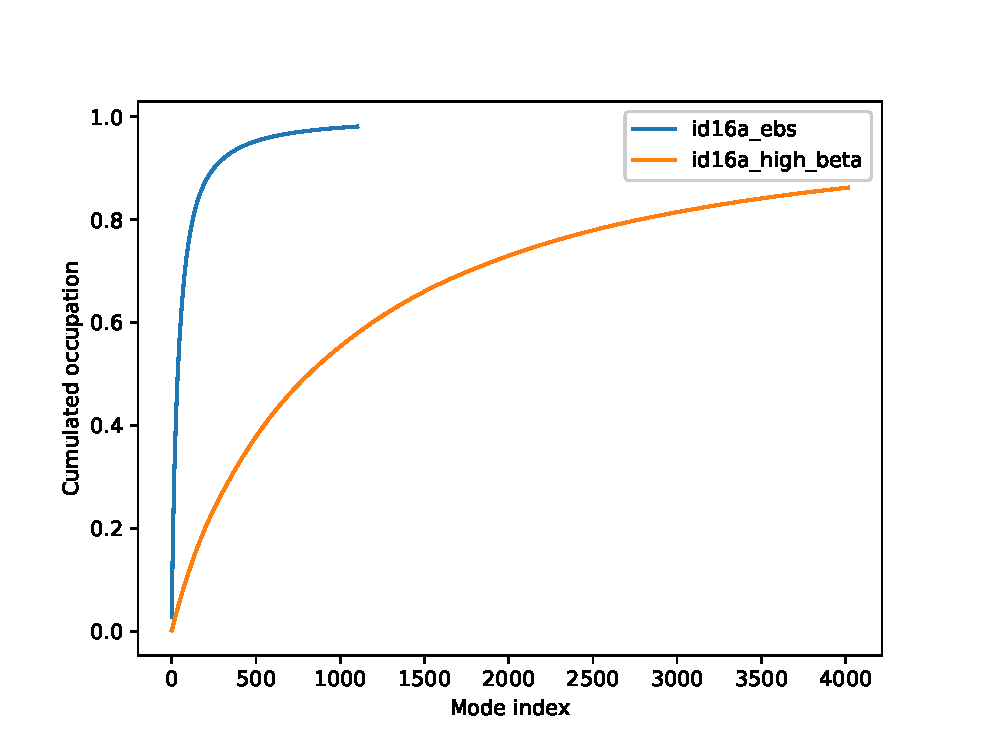
\includegraphics[width=7cm]{GRAPHICS/cumulated_occupation.eps}
        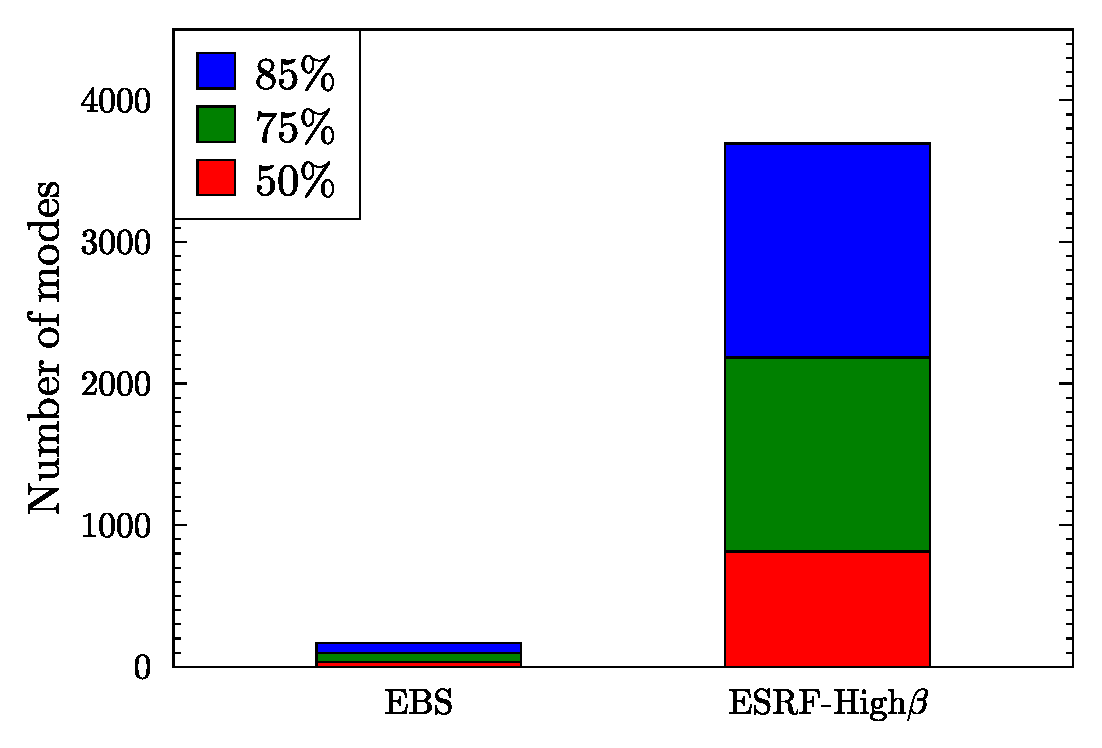
\includegraphics[width=6.5cm]{GRAPHICS/up_to_mode_id16a.eps}
    \caption{Cumulated occupation of the coherent modes for the EBS and ESRF-High-$\beta$ (top), and number of modes needed to reach a given percent of CSD occupation (bottom). }
\end{figure}

The spectral density at the EBS photon source is represented in Fig.~\ref{fig:spectraldensity}a. It shows an elliptical shape with horizontal size larger than the vertical.  The spectral density is reproduced by the addition of the coherent modes weighted by the eigenvectors (from Eq.~\ref{decomposition})
\begin{equation}
S(x,y) = \sum_{m=0}^{\infty} \lambda_m |\Phi_m(x,y)|^2.
\end{equation}
Figs.~\ref{fig:spectraldensity}b-e represent the coherent modes with $m$=0 to $m$=3. It can be shown that the first mode is centered on the axis but extends over an spatial region smaller than the spectral density. Next mode ($m$=1) contributes to extend the spectral density in horizontal, but presents zero intensity at the origin. Successive modes extend  the spectral density in horizontal, sometimes presenting a lobe centerer at zero and sometimes not (e.g., $m$=3). Modes with several lobes along the vertical will also appear, but not so often than in the horizontal, because of the elliptical shape of the spectral density. The coherent modes are orthonormal, thus verifying 
\begin{equation}\label{eq:mode normalization}
M_{mn} = \int_{-\infty}^{\infty} \Phi^*_m(x,y) \Phi_n(x,y)~dx~dy = \delta_{mn}
\end{equation}
with $\delta_{mn}$ the Kronecker delta. The coherence fraction of 2.8\% for the EBS source means that for an optimal coherence experiment one should remove 97.2\% of the emitted photons. This task is performed by the beamline. The beamline elements modify the different modes in a different manner, but it will never be possible to remove all the photons except from the lowest coherent mode, because there is an overlapping of the intensity of the lowest mode with the other ones. Therefore it is impossible to obtain a fully coherent beam that must contain only a single mode. 

   



\begin{figure}\label{fig:spectraldensity}
    \centering
        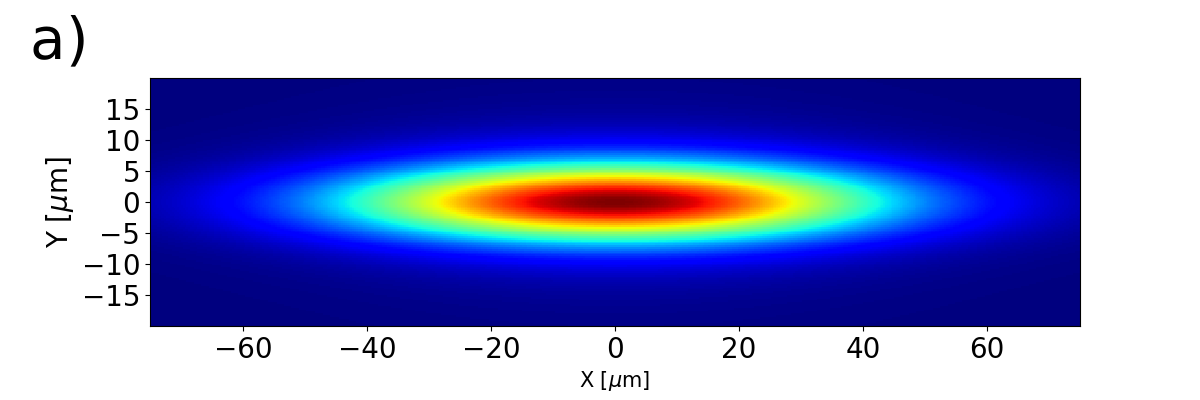
\includegraphics[width=\textwidth]{GRAPHICS/ebs_spectral_density.png}
        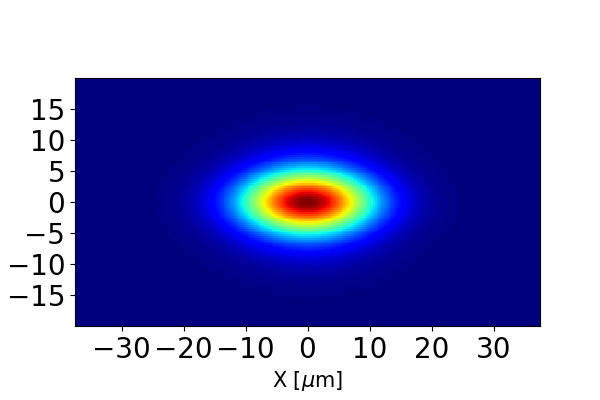
\includegraphics[width=0.45\textwidth]{GRAPHICS/ebs_mode0.png}
        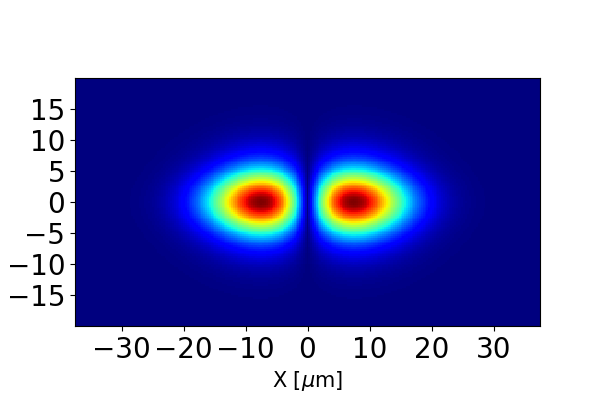
\includegraphics[width=0.45\textwidth]{GRAPHICS/ebs_mode1.png}
        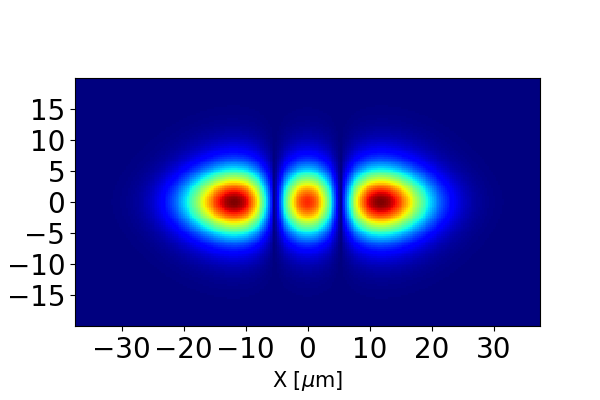
\includegraphics[width=0.45\textwidth]{GRAPHICS/ebs_mode2.png}
        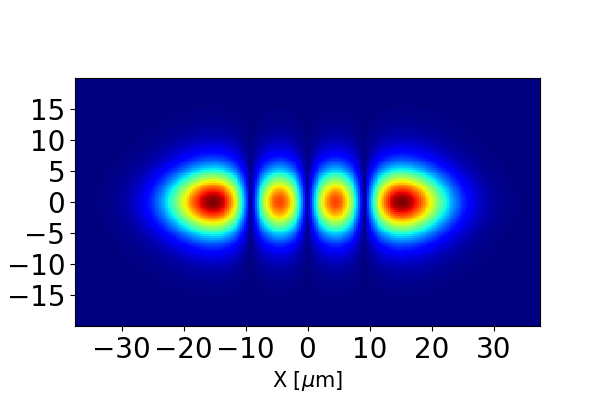
\includegraphics[width=0.45\textwidth]{GRAPHICS/ebs_mode3.png}
    \caption{a) Spectral density $S(x,y)$ at the source position for EBS.  }
\end{figure}


The coherent modes calculated at the EBS source have been propagated using a beamline simplified with ideal focusing elements and slits to determine their numerical aperture (like in Section~\ref{wofry}). Fig.~\ref{fig:mode transmission} shows how the intensity of the first modes is reduced by geometrical considerations. 
%We recall that in the coherent mode expansion, the modes are orthonormal, therefore the integrated intensity for any mode is always one at the source. 
As discussed, coherent modes will be ``cut'' in a different manner, depending on the slits cropping effect.
This imply that the Eq.~\ref{eq:mode normalization} is not longer verified, and for the propagated modes $M_{mm}\le$1 and $M_{mn}\ne$0 for $m\ne n$. Therefore, the coherent modes of the source after propagation and cropping by the beamline are no longer coherent modes of the resulting beam. Fig.~\ref{fig:mode transmission} shows that the most important transfer ratio ($M_{mm}$)transfer for the lowest mode is about $M_{00}$=25\%, then $M_{22}$=10\% and $M_{44}$=6\%. The other modes shown transfer less than 5\% transfer, and modes higher than $m$=10 practically do not contribute to the final spectral density. Note that, as discussed before, the transmission of mode $m$=2 is higher than mode $m$=1, because this one does not contain a central lobe (Fig.~\ref{fig:spectraldensity}c).  

% #########################################################
%            iteration            intensity         intensity/I0   intensity/TotalInt
%                    0               0.23967               1.00000              0.44091 
%                    1              0.022004               0.09181              0.04048 
%                    2               0.10008               0.41757              0.18411 
%                    3              0.028309               0.11812              0.05208 
%                    4              0.061262               0.25561              0.11270 
%                    5              0.026262               0.10958              0.04831 
%                    6               0.03452               0.14403              0.06351 
%                    7               0.01459               0.06087              0.02684 
%                    8              0.011714               0.04887              0.02155 
%                    9             0.0051714               0.02158              0.00951

% #########################################################
%            iteration            intensity         intensity/I0   intensity/TotalInt
%                    0            1.0793e+06               1.00000              0.49537 
%                    1                 93290               0.08644              0.04282 
%                    2            3.9938e+05               0.37004              0.18331 
%                    3            1.0632e+05               0.09851              0.04880 
%                    4            2.1648e+05               0.20058              0.09936 
%                    5                 87305               0.08089              0.04007 
%                    6            1.0794e+05               0.10001              0.04954 
%                    7                 42906               0.03975              0.01969 
%                    8                 32393               0.03001              0.01487 
%                    9                 13446               0.01246              0.00617 

\begin{figure}\label{fig:mode transmission}
    \centering
        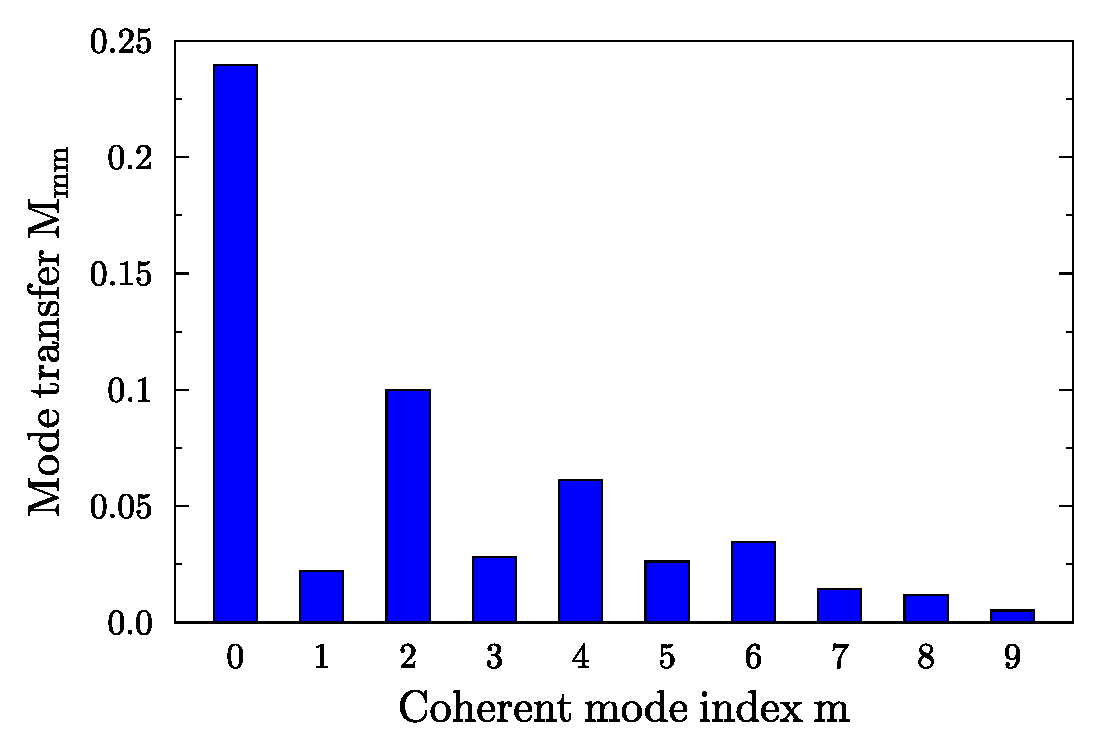
\includegraphics[width=\textwidth]{GRAPHICS/propagated_modes.eps}
    \caption{Transmission $M_{mm}$ (see Eq.~\ref{eq:mode normalization}) of the different modes of the EBS source  due to the effect of propagation and cropping by the beamline optics.}
\end{figure}

This analysis of the mode transmission is mode dramatic if one looks to the total intensity in the mode, which is given by its eigenvalue. Neglecting modes higher than 10, the lowest coherent mode ($m$=0) carries the 49.5\% of the beam intensity, 18.4\% for the mode $m$=2, and less than 5\% for the others. 

% 0    8.283396938003417809e-01
% 1    1.334192926516760969e-01
% 2    1.726189402927864533e-02
% 3    7.157008449213129661e-03
% 4    6.639480916324663404e-03
% 5    3.894724551090737296e-03
% 6    2.436986236753659139e-03
% 7    4.732687905858104635e-04
% 8    2.758652782324634112e-04
% 9    7.761681183345831123e-05
% 10   1.934547528193778418e-05

\begin{figure}\label{fig:rediagonalization}
    \centering
        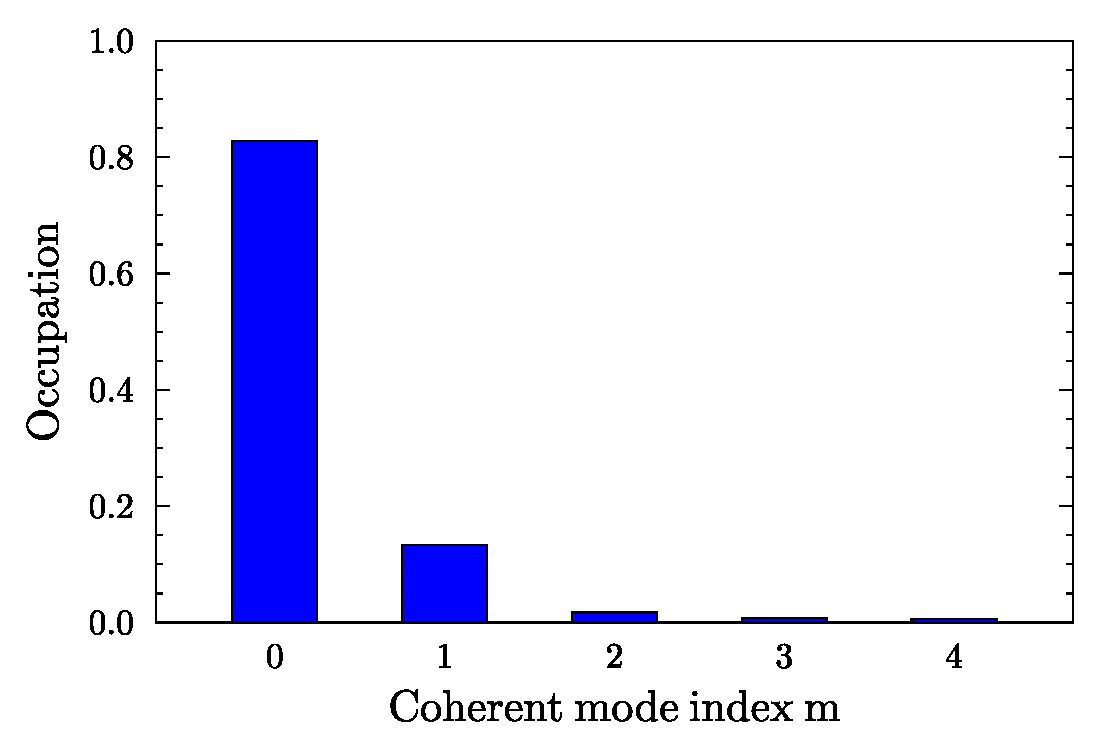
\includegraphics[width=\textwidth]{GRAPHICS/rediagonalized_modes.eps}
    \caption{Occupation of the coherent modes of the final focused beam.}
\end{figure}

As commented before, the coherent modes at the source, propagated and cropped by the beamline, are not longer orthonormal, therefore they cannot be called coherent modes of the resulting beam. At this point, the new coherent modes can be calculated applying a new coherent mode decomposition on the cross spectral density of the transmitted beam, that is known from source coherent mode expansion. Making this numerical calculation with COMSYL, one obtains a mode occupation spectrum (see Fig.~\ref{fig:rediagonalization}) where the lowest mode accounts for the 83\% of the total spectral density. The next mode accounts for only 13\% and the rest are practically negligeable. The intensity of these two coherent modes is shown in Fig.~\ref{fig:final modes}. The first mode has FWHM dimensions of 7.3$\times$6.7 nm$^2$. The spectral density, that is practically given by the contribution of the first two modes has a FWHM equal to the $m$=0 mode because, in horizontal the $m$=1 mode does contribute only to the tails and in vertical is identical to mode $m$=0.

This analysis confirms the quantitative predictions discussed in the previous sections, but give a quantitative figure of the coherence of the beam, a  coherent fraction of CF=83\% that measures the "coherence purity".


 




\begin{figure}\label{fig:final modes}
    \centering
        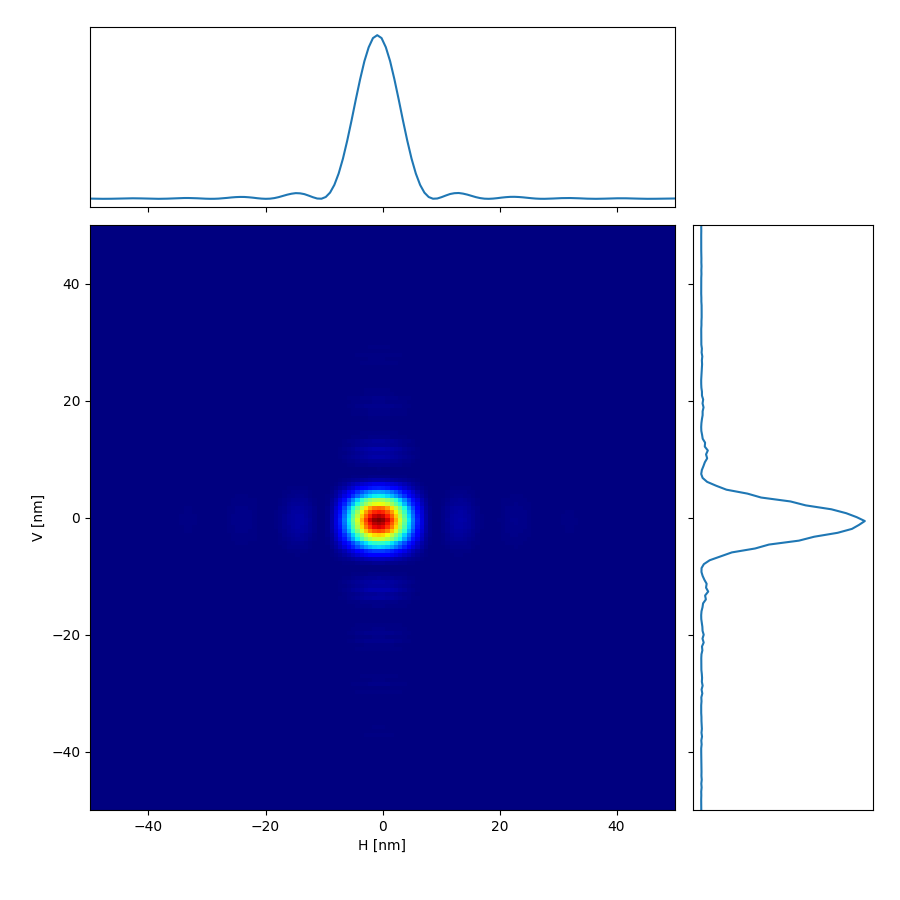
\includegraphics[width=0.95\textwidth]{GRAPHICS/final_mode0.png}
        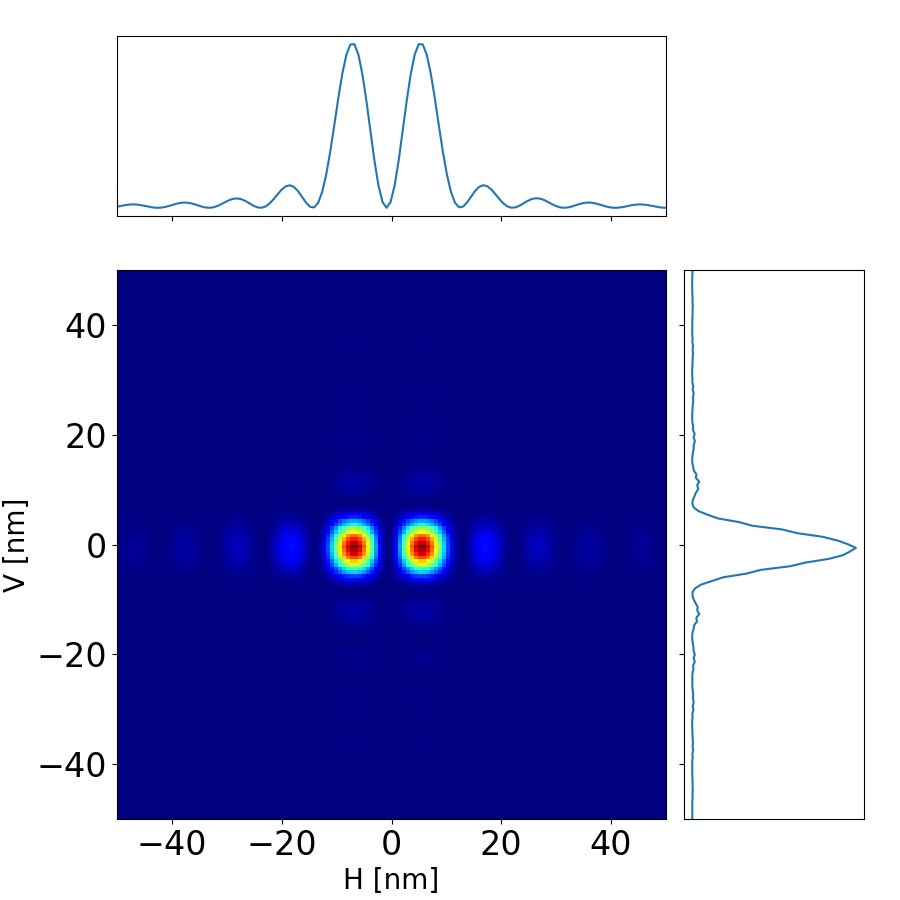
\includegraphics[width=0.95\textwidth]{GRAPHICS/final_mode1.png}
    \caption{Coherent modes of the focused beam. Top: lower mode ($m$=0), with 83\% occupation and FWHM of 7.3$\times$6.7 nm$^2$. Botton: mode $m$=1, with 13\% occupation and FWHM of 19.0$\times$6.7 nm$^2$}
\end{figure}


\todo{
\begin{itemize}
 \item introduce slope errors in WOFRY propagation
 \item propagate modes with SRW
 \item create some plots with cuts of W
\end{itemize}
}
 

\section{Discussion} 
\label{discussion}

After the complete analysis done in the previous section on how the ID16A optics modify the characteristics of the x-ray beam, one can verify that the analytical previsions were a good estimator of the values then obtained using more sophisticated methods. The size of the focused beam (e.g, 10x5 for EBS) and the transmission (3\%) calculated analytically are in good agreement with geometric ray tracing (8.4x4.8, and 2.28\%). When characterising beam sizes, one usually assume that the intensity distributions are Gaussian and therefore they are well characterised by the FWHM value. From Fig.~\ref{fig:ray tracing} one can see that the horizontal intensity distribution is not Gaussian for the ESRF, as a result of cropping the beam with the VSS opened to 50$\mu$m. Although the electron beam statistics is in a very good approximations Gaussian, the undulator emission is not. In our ray tracing simulations we always suppose that we work at the resonance, then we applied the Gaussian approximation used in Eqs.~\ref{eq:photon small sigmas} and \ref{eq:photon big sigmas} to compute the geometrical characteristics of the source. This is certainly acceptable at the resonance but will fail out of resonance. Indeed, these lack of Gaussianity is relevant in the calculations of the coherent fraction. We approximate the coherence fraction by Eq.~\ref{eq:coherent fraction}, which for zero emittance ($\sigma_{x,y}=\sigma_{x',y'}$=0) becomes CF=1, as expected because a zero emittance electron beam (a single electron or a filament beam) that travel in an magnetic field emits a fully coherent wavefront. However, the photon source for a filament beam would have an emittance of $\sigma_u \sigma_{u'} \approx \lambda / 2 \pi$ (using Eqs.~\ref{eq:photon small sigmas}), which is in contradiction with theory, that says that a pure coherent state has emittance of $\lambda / 4 \pi$, as happens for a Gaussian photon beam. This is justified considering that Eqs.~\ref{eq:photon small sigmas} are approximations obtained by fitting with Gaussians the theoretical non-Gaussian distributions (see Ref.~\cite{elleaume}). The correct definition of CF as the occupation of the lowest coherent mode does not present these incongruences. However, its calculation requires to perform the coherent mode decomposition, as done in Section~\ref{comsyl} which is very costly. It is therefore the case to find the compromise between accuracy and cost, or where in the hierarchical series of methodologies proposed one should stop. 

The combination of ray tracing and wave optics methods used indicate that the focalized beam size due to  demagnification with mirrors (giving for EBS 10x5 nm2 analytically, 8.4x4.8 nm2 with ray tracing) has to be corrected with diffraction effect (8.4x7.8 hybrid, 12.7x9.2 SRW) and then add the slope error effect. The slope errors are very small, necessary not to blow up the size and kit it in the specifications range (10.8x8.2 hybrid 13.6x9.9 SRW). It is important to treat the the slope errors correctly. Slope errors can be included in the ray tracing using the data in Appendix A and applying specular reflection on the optical surface with errors. This is the standard mode of including slope errors in SHADOW, using measured profiles or synthetic ones. It works well for the case of incoherent beams, but in our case, because of the high coherence of the beam the ray tracing method (specular reflection) overestimates the blowing of the focal spot conducting to wrong results. Therefore the slope errors of the KB system have been considered using a ``wave optics approach'', as explained in Ref.~\cite{hybrid}. Here, the mirror height errors $z(x)$ are projected to the plane perpendicular to the propagation ($z(x) \sin \theta$, with $\theta$ the grazing angle). They introduce a phase shift $\psi$ in the wavefront phase proportional to the optical path $\psi = - k z(x) \sin \theta $. This is the algorithm used in the simulations in Sections~\ref{level1}, \ref{srw_se} and \ref{srw_me}.   


% The first step in the wave optics simulation is to assume a full coherent source and simulate the propagation of such wavefront through the beamline. 

The wavefront simulation of the beamline include propagation of the beam from element to element (drift spaces) using different possible propagators. A propagator based on the Freskel-Kirchhoff integral is used. The applications of this (and other) operators imply the calculation of an integral (or sum) at each pixel of the image plane. This is costly from the computer point of view, so Fourier Transforms (Fourier Optics) and its Fast Fourier Transform implementation are used to reduce amount of operations and the calculation time. This is practically the only choice for propagating 2D wavefronts. The use of Fourier Transforms adds another problem: the result is very dependent on the sampling of the wavefront (i.e., pixel size, number of points, dimension of the window where the wavefront is defined). This means the usually one has to test many configurations before finding one that works reasonably well (even though one can never guarantee the complete accuracy of the sampling used). A full wavefront optics simulation is an iterative process, where the user has to refine the sampling parameters element by element to be sure the wavefront at each position is sampled correctly. This is a time consuming work in particular for 2D simulation. We found very useful to start a wavefront simulation in 1D, separating the horizontal and vertical simulations, using a simplified system with ideal sources and ideal focusing elements. The use of 1D propagation is justified because in in synchrotron beamlines the horizontal and vertical coupling is usually small. This 1D simulations help in refining the choice of propagator and its parameters (resampling, zoom factors) that can be reused in a full 2D simulations.

Regarding computational effort, simulations concerning ray tracing (Section~\ref{level1}) and coherent optics (Sections~\ref{wofry} and \ref{srw_se}) can be done interactively in a normal laptop. However, for those concerning partial coherence, very long calculations are needed. For example, Monte Carlo calculations in Section~\ref{srw_me} for the multi electron case \inred{HOW MANY ELECTRONS?} spent a few hours on a 56-core computer cluster. For performing the COMSYL coherent mode decomposition the calculation time depends very much on the dimensions on the problem. For EBS the wavefronts were sampled using 1007x335 pixels, and 1103 modes were computed representing 98\% of the spectral density. This represents 5 MB per wavefront and a matrix of 1695 GB to diagonalize. It took less that four hours in the a cluster of 28 cores. The calculation is more expensive if one wants to decompose a source that is pretty incoherent like our ESRF-High-$\beta$. This is a limit case, it was used wavefields of XxX pixels to accommodate the large spatial extension of the source. The calculation took XX days in a large XX cluster. 
%To give an idea of the real cost, a similar work send to the AWS cluster costed about 2000 USD. 
This was done as a test case, to demonstrate the feasibility of the calculations. It is not recommended to do similar calculations that imply a the cost because a source that is quite incoherent was treated with partial coherence methods. In Appendix B we present for the ESRF High$\beta$ similar results than those in Section~\ref{comsyl}. 

Some effects that are typically studied when designing and simulating a beamline have not been discussed here. For example the study of the power emitted by the source and its heat load effect in the first (or firsts) slits and optical elements (here the ML monochromator). Also, the reflectivity of the elements are not considered. The simulation of this was not included in the simulations, because it can be estimated analytically considering an average reflectivity about \inred{0.7 for multilayers and 0.9 for mirrors, therefore a reduction factor of (0.7)**3 ML for the beamline flux due to reflectivity of mirror coatings}. 

\todo{discuss coherence length}


\section{Summary and conclusions}

We have obtained quantitative values of flux, transmission, size of the focused beam, and coherent fraction for ID16A, a modern beamline with already exceptional performances in terms of nanofucusing and coherence. We predicted advances the improvements in these parameters when the EBS will start in 2020. We obtained these parameters using a hierarchical flowchart with, applying methods with increasing complexity and requiring higher computational effort. 

The analytical estimation of the main parameters is mandatory first step in the beamline conception and analysis. We applied concepts based on optical magnification and numerical aperture acceptance and calculated approximately the coherent fraction at the source. These values help to perform sanity check of the computer simulations. A ray tracing simulation is inexpensive and provides important information. The comparison of the CF with the beamline transmitivity would give an idea of the beam coherence, reflected in the number modes present in the final beam. For high coherence, like for ID16A, the wave optics calculations are necessary. If the final beam has a very high coherence, like in our case, coherent optics (1D simplifications, and single electron calculations) may give good results. Full calculations based on coherent mode decomposition Were introduced here. It is a new way of quantitatively assess the quality of the partial coherent beam via the calculation of the coherent modes of the source, propagation of the modes and recalculating the coherent mode expansion on the final beam from which one obtains the CF, a parameter that valutated the coherence quality. 




% It is interesting to remark that although Monte Carlo multielectron method can in principle calculate Eq.~\ref{CSD} the storage at every point is unmanagleable, so usually only some 'cuts' of the CSD are stored, such as $W(x_1,0,x_2,0;z,\omega)$ (horizontal) or $W(0,y_1,0,y_2;z,\omega)$ (vertical) \todo{move this to the discussion?}.
% 
% 
% The fist coherence mode is always centered on-axis (see, e.g, Fig.~\ref{fig:spectraldensity}b) and will always be centered when propagated until a position where an optical element (an aperture or mirror with finite dimensions) will crop it removing part of its intensity but letting the central part to go throught. The subsequent modes will be more absorbed as they extend more. In particular the modes that do not have a central lobe will lose more intensity. 


\todo{
\begin{itemize}
 \item comment on the heat-load deformation 
 \item comment the effect of reflectivity by ML and mirror coating
 \item comment on the main results in terms of intensity and size
 \item EXPERIMENTAL RESULTS?
 \item comment ``where to stop'' in a simulation, depending on the level of accuracy requested
 \item comment on the computer resources used for simulations
 \item comment on software tools: OASYS (and make a graphic)
 \item discuss the particularities of this beamline 
 \item comment on general strategy for beamline simulations and the application of the shown hierarchical model. Make a flowchart
\end{itemize}
}

\ack{\todo{someone to thank?}}

\appendix

\section{Metrology of the KB mirrors}

\section{COMSYL results for the ESRF-H$\beta$}



\bibliographystyle{iucr}
\bibliography{paper-hierarchical}


\end{document}                    % DO NOT DELETE THIS LINE
%%%%%%%%%%%%%%%%%%%%%%%%%%%%%%%%%%%%%%%%%%%%%%%%%%%%%%%%%%%%%%%%%%%%%%%%%%%%%%
